\documentclass[twoside]{book}

% Packages required by doxygen
\usepackage{fixltx2e}
\usepackage{calc}
\usepackage{doxygen}
\usepackage[export]{adjustbox} % also loads graphicx
\usepackage{graphicx}
\usepackage[utf8]{inputenc}
\usepackage{makeidx}
\usepackage{multicol}
\usepackage{multirow}
\PassOptionsToPackage{warn}{textcomp}
\usepackage{textcomp}
\usepackage[nointegrals]{wasysym}
\usepackage[table]{xcolor}

% NLS support packages
\usepackage[spanish]{babel}
% Font selection
\usepackage[T1]{fontenc}
\usepackage[scaled=.90]{helvet}
\usepackage{courier}
\usepackage{amssymb}
\usepackage{sectsty}
\renewcommand{\familydefault}{\sfdefault}
\allsectionsfont{%
  \fontseries{bc}\selectfont%
  \color{darkgray}%
}
\renewcommand{\DoxyLabelFont}{%
  \fontseries{bc}\selectfont%
  \color{darkgray}%
}
\newcommand{\+}{\discretionary{\mbox{\scriptsize$\hookleftarrow$}}{}{}}

% Page & text layout
\usepackage{geometry}
\geometry{%
  a4paper,%
  top=2.5cm,%
  bottom=2.5cm,%
  left=2.5cm,%
  right=2.5cm%
}
\tolerance=750
\hfuzz=15pt
\hbadness=750
\setlength{\emergencystretch}{15pt}
\setlength{\parindent}{0cm}
\setlength{\parskip}{3ex plus 2ex minus 2ex}
\makeatletter
\renewcommand{\paragraph}{%
  \@startsection{paragraph}{4}{0ex}{-1.0ex}{1.0ex}{%
    \normalfont\normalsize\bfseries\SS@parafont%
  }%
}
\renewcommand{\subparagraph}{%
  \@startsection{subparagraph}{5}{0ex}{-1.0ex}{1.0ex}{%
    \normalfont\normalsize\bfseries\SS@subparafont%
  }%
}
\makeatother

% Headers & footers
\usepackage{fancyhdr}
\pagestyle{fancyplain}
\fancyhead[LE]{\fancyplain{}{\bfseries\thepage}}
\fancyhead[CE]{\fancyplain{}{}}
\fancyhead[RE]{\fancyplain{}{\bfseries\leftmark}}
\fancyhead[LO]{\fancyplain{}{\bfseries\rightmark}}
\fancyhead[CO]{\fancyplain{}{}}
\fancyhead[RO]{\fancyplain{}{\bfseries\thepage}}
\fancyfoot[LE]{\fancyplain{}{}}
\fancyfoot[CE]{\fancyplain{}{}}
\fancyfoot[RE]{\fancyplain{}{\bfseries\scriptsize Generado por Doxygen }}
\fancyfoot[LO]{\fancyplain{}{\bfseries\scriptsize Generado por Doxygen }}
\fancyfoot[CO]{\fancyplain{}{}}
\fancyfoot[RO]{\fancyplain{}{}}
\renewcommand{\footrulewidth}{0.4pt}
\renewcommand{\chaptermark}[1]{%
  \markboth{#1}{}%
}
\renewcommand{\sectionmark}[1]{%
  \markright{\thesection\ #1}%
}

% Indices & bibliography
\usepackage{natbib}
\usepackage[titles]{tocloft}
\setcounter{tocdepth}{3}
\setcounter{secnumdepth}{5}
\makeindex

% Hyperlinks (required, but should be loaded last)
\usepackage{ifpdf}
\ifpdf
  \usepackage[pdftex,pagebackref=true]{hyperref}
\else
  \usepackage[ps2pdf,pagebackref=true]{hyperref}
\fi
\hypersetup{%
  colorlinks=true,%
  linkcolor=blue,%
  citecolor=blue,%
  unicode%
}

% Custom commands
\newcommand{\clearemptydoublepage}{%
  \newpage{\pagestyle{empty}\cleardoublepage}%
}

\usepackage{caption}
\captionsetup{labelsep=space,justification=centering,font={bf},singlelinecheck=off,skip=4pt,position=top}

%===== C O N T E N T S =====

\begin{document}

% Titlepage & ToC
\hypersetup{pageanchor=false,
             bookmarksnumbered=true,
             pdfencoding=unicode
            }
\pagenumbering{alph}
\begin{titlepage}
\vspace*{7cm}
\begin{center}%
{\Large My Project }\\
\vspace*{1cm}
{\large Generado por Doxygen 1.8.13}\\
\end{center}
\end{titlepage}
\clearemptydoublepage
\pagenumbering{roman}
\tableofcontents
\clearemptydoublepage
\pagenumbering{arabic}
\hypersetup{pageanchor=true}

%--- Begin generated contents ---
\chapter{Indice jerárquico}
\section{Jerarquía de la clase}
Esta lista de herencias esta ordenada aproximadamente por orden alfabético\+:\begin{DoxyCompactList}
\item \contentsline{section}{Database\+Handler}{\pageref{classDatabaseHandler}}{}
\item \contentsline{section}{Heroku\+Service}{\pageref{classHerokuService}}{}
\item Json\+Controller\begin{DoxyCompactList}
\item \contentsline{section}{Api\+Json\+Controller}{\pageref{classApiJsonController}}{}
\end{DoxyCompactList}
\item \contentsline{section}{Log}{\pageref{classLog}}{}
\item \contentsline{section}{M\+D5}{\pageref{classMD5}}{}
\item \contentsline{section}{Order\+By\+Votes}{\pageref{structOrderByVotes}}{}
\item \contentsline{section}{User}{\pageref{classUser}}{}
\item \contentsline{section}{User\+Handler}{\pageref{classUserHandler}}{}
\item \contentsline{section}{User\+List}{\pageref{classUserList}}{}
\item Web\+Controller\begin{DoxyCompactList}
\item \contentsline{section}{Linkedin\+Web\+Controller}{\pageref{classLinkedinWebController}}{}
\end{DoxyCompactList}
\end{DoxyCompactList}

\chapter{Índice de clases}
\section{Lista de clases}
Lista de las clases, estructuras, uniones e interfaces con una breve descripción\+:\begin{DoxyCompactList}
\item\contentsline{section}{\hyperlink{classApiJsonController}{Api\+Json\+Controller} }{\pageref{classApiJsonController}}{}
\item\contentsline{section}{\hyperlink{classDatabaseHandler}{Database\+Handler} }{\pageref{classDatabaseHandler}}{}
\item\contentsline{section}{\hyperlink{classHerokuService}{Heroku\+Service} }{\pageref{classHerokuService}}{}
\item\contentsline{section}{\hyperlink{classLinkedinWebController}{Linkedin\+Web\+Controller} }{\pageref{classLinkedinWebController}}{}
\item\contentsline{section}{\hyperlink{classLog}{Log} }{\pageref{classLog}}{}
\item\contentsline{section}{\hyperlink{classMD5}{M\+D5} }{\pageref{classMD5}}{}
\item\contentsline{section}{\hyperlink{structOrderByVotes}{Order\+By\+Votes} }{\pageref{structOrderByVotes}}{}
\item\contentsline{section}{\hyperlink{classUser}{User} }{\pageref{classUser}}{}
\item\contentsline{section}{\hyperlink{classUserHandler}{User\+Handler} }{\pageref{classUserHandler}}{}
\item\contentsline{section}{\hyperlink{classUserList}{User\+List} }{\pageref{classUserList}}{}
\end{DoxyCompactList}

\chapter{Indice de archivos}
\section{Lista de archivos}
Lista de todos los archivos con descripciones breves\+:\begin{DoxyCompactList}
\item\contentsline{section}{/home/ezequiel/taller2/taller2/server/src/\hyperlink{ApiJsonController_8cpp}{Api\+Json\+Controller.\+cpp} }{\pageref{ApiJsonController_8cpp}}{}
\item\contentsline{section}{/home/ezequiel/taller2/taller2/server/src/\hyperlink{ApiJsonController_8h}{Api\+Json\+Controller.\+h} }{\pageref{ApiJsonController_8h}}{}
\item\contentsline{section}{/home/ezequiel/taller2/taller2/server/src/\hyperlink{base64_8cpp}{base64.\+cpp} }{\pageref{base64_8cpp}}{}
\item\contentsline{section}{/home/ezequiel/taller2/taller2/server/src/\hyperlink{base64_8h}{base64.\+h} }{\pageref{base64_8h}}{}
\item\contentsline{section}{/home/ezequiel/taller2/taller2/server/src/\hyperlink{DatabaseHandler_8cpp}{Database\+Handler.\+cpp} }{\pageref{DatabaseHandler_8cpp}}{}
\item\contentsline{section}{/home/ezequiel/taller2/taller2/server/src/\hyperlink{DatabaseHandler_8h}{Database\+Handler.\+h} }{\pageref{DatabaseHandler_8h}}{}
\item\contentsline{section}{/home/ezequiel/taller2/taller2/server/src/\hyperlink{HerokuService_8cpp}{Heroku\+Service.\+cpp} }{\pageref{HerokuService_8cpp}}{}
\item\contentsline{section}{/home/ezequiel/taller2/taller2/server/src/\hyperlink{HerokuService_8h}{Heroku\+Service.\+h} }{\pageref{HerokuService_8h}}{}
\item\contentsline{section}{/home/ezequiel/taller2/taller2/server/src/\hyperlink{LinkedinWebController_8cpp}{Linkedin\+Web\+Controller.\+cpp} }{\pageref{LinkedinWebController_8cpp}}{}
\item\contentsline{section}{/home/ezequiel/taller2/taller2/server/src/\hyperlink{LinkedinWebController_8h}{Linkedin\+Web\+Controller.\+h} }{\pageref{LinkedinWebController_8h}}{}
\item\contentsline{section}{/home/ezequiel/taller2/taller2/server/src/\hyperlink{log_8cpp}{log.\+cpp} }{\pageref{log_8cpp}}{}
\item\contentsline{section}{/home/ezequiel/taller2/taller2/server/src/\hyperlink{log_8h}{log.\+h} }{\pageref{log_8h}}{}
\item\contentsline{section}{/home/ezequiel/taller2/taller2/server/src/\hyperlink{main_8cpp}{main.\+cpp} }{\pageref{main_8cpp}}{}
\item\contentsline{section}{/home/ezequiel/taller2/taller2/server/src/\hyperlink{md5_8cpp}{md5.\+cpp} }{\pageref{md5_8cpp}}{}
\item\contentsline{section}{/home/ezequiel/taller2/taller2/server/src/\hyperlink{md5_8h}{md5.\+h} }{\pageref{md5_8h}}{}
\item\contentsline{section}{/home/ezequiel/taller2/taller2/server/src/\hyperlink{User_8cpp}{User.\+cpp} }{\pageref{User_8cpp}}{}
\item\contentsline{section}{/home/ezequiel/taller2/taller2/server/src/\hyperlink{User_8h}{User.\+h} }{\pageref{User_8h}}{}
\item\contentsline{section}{/home/ezequiel/taller2/taller2/server/src/\hyperlink{UserHandler_8cpp}{User\+Handler.\+cpp} }{\pageref{UserHandler_8cpp}}{}
\item\contentsline{section}{/home/ezequiel/taller2/taller2/server/src/\hyperlink{UserHandler_8h}{User\+Handler.\+h} }{\pageref{UserHandler_8h}}{}
\item\contentsline{section}{/home/ezequiel/taller2/taller2/server/src/\hyperlink{UserList_8cpp}{User\+List.\+cpp} }{\pageref{UserList_8cpp}}{}
\item\contentsline{section}{/home/ezequiel/taller2/taller2/server/src/\hyperlink{UserList_8h}{User\+List.\+h} }{\pageref{UserList_8h}}{}
\end{DoxyCompactList}

\chapter{Documentación de las clases}
\hypertarget{classApiJsonController}{}\section{Referencia de la Clase Api\+Json\+Controller}
\label{classApiJsonController}\index{Api\+Json\+Controller@{Api\+Json\+Controller}}


{\ttfamily \#include $<$Api\+Json\+Controller.\+h$>$}

Diagrama de herencias de Api\+Json\+Controller\begin{figure}[H]
\begin{center}
\leavevmode
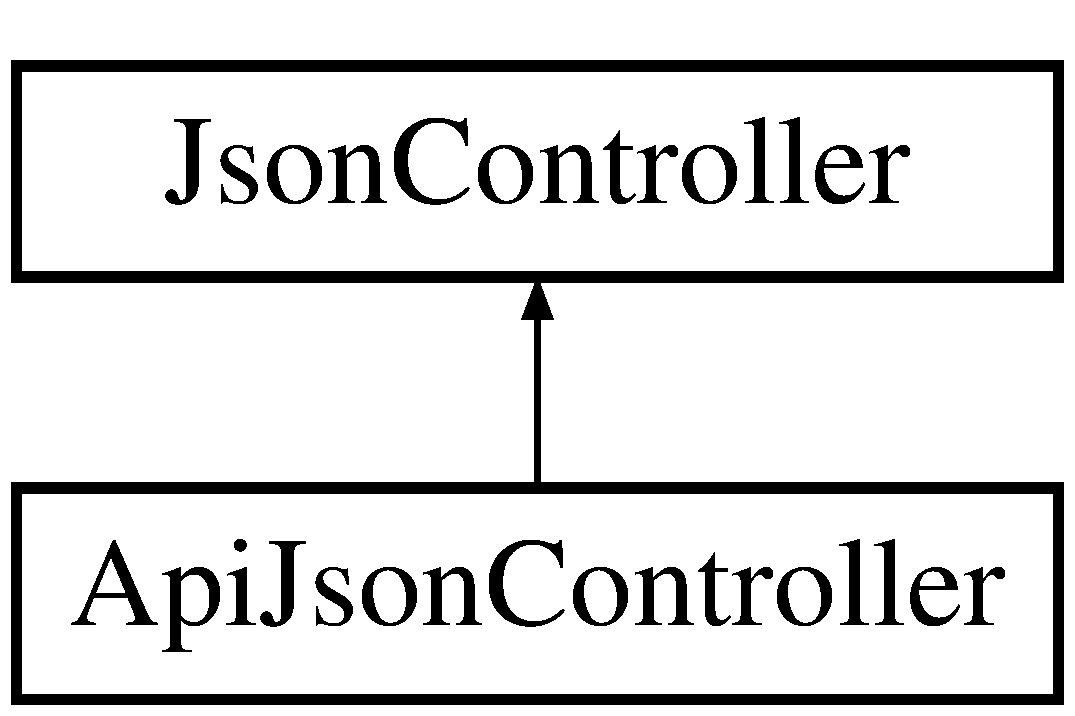
\includegraphics[height=2.000000cm]{classApiJsonController}
\end{center}
\end{figure}
\subsection*{Métodos públicos}
\begin{DoxyCompactItemize}
\item 
\hyperlink{classApiJsonController_ad5d1aff126905ea4a9cc85d481e747a0}{Api\+Json\+Controller} ()
\item 
\hyperlink{classApiJsonController_a889add94a7d9a5a5e0cb4278fa81eb47}{$\sim$\+Api\+Json\+Controller} ()
\item 
virtual void \hyperlink{classApiJsonController_a1e809af244d7c98b3033e573919921b2}{setup} ()
\item 
void \hyperlink{classApiJsonController_adef3856c8f8f6cc7f4d980c31a9c31fb}{hello} (Mongoose\+::\+Request \&request, Mongoose\+::\+Json\+Response \&response)
\item 
void \hyperlink{classApiJsonController_a51551fd5eb0a87f79f810d67353584cb}{testdb} (Mongoose\+::\+Request \&request, Mongoose\+::\+Json\+Response \&response)
\item 
void \hyperlink{classApiJsonController_a6f3831b46ccd2b684256d8475de08e50}{login} (Mongoose\+::\+Request \&request, Mongoose\+::\+Json\+Response \&response)
\item 
void \hyperlink{classApiJsonController_adc58c5ee867cd7ebd906a93c2ab66e23}{logout} (Mongoose\+::\+Request \&request, Mongoose\+::\+Json\+Response \&response)
\item 
void \hyperlink{classApiJsonController_ae31f4111016a43bf025c513ab7d7a6be}{job\+\_\+positions} (Mongoose\+::\+Request \&request, Mongoose\+::\+Json\+Response \&response)
\item 
void \hyperlink{classApiJsonController_a517f518559e86d3b5d1ce962a187694e}{categories} (Mongoose\+::\+Request \&request, Mongoose\+::\+Json\+Response \&response)
\item 
void \hyperlink{classApiJsonController_a2d2a0b94bcf49ece8444ef3b30a61189}{skills} (Mongoose\+::\+Request \&request, Mongoose\+::\+Json\+Response \&response)
\item 
void \hyperlink{classApiJsonController_aa0ae8d88ab73349b5cbebea85127e485}{my\+\_\+profile} (Mongoose\+::\+Request \&request, Mongoose\+::\+Json\+Response \&response)
\item 
void \hyperlink{classApiJsonController_a4e1c8c117457100c5297cfac507e78ef}{fb\+\_\+login} (Mongoose\+::\+Request \&request, Mongoose\+::\+Json\+Response \&response)
\item 
void \hyperlink{classApiJsonController_aaac98bdb7d1dc373db45f81cde5a2ba1}{edit} (Mongoose\+::\+Request \&request, Mongoose\+::\+Json\+Response \&response)
\item 
void \hyperlink{classApiJsonController_a56784a6400512fb7d2cdf499b7f60005}{new\+\_\+user} (Mongoose\+::\+Request \&request, Mongoose\+::\+Json\+Response \&response)
\item 
void \hyperlink{classApiJsonController_ae4c1ff09c9e16db375ea371086b45e5b}{add\+\_\+contact} (Mongoose\+::\+Request \&request, Mongoose\+::\+Json\+Response \&response)
\item 
void \hyperlink{classApiJsonController_aa68f90e0aa81f847afbfb55764eac073}{answer\+\_\+contact} (Mongoose\+::\+Request \&request, Mongoose\+::\+Json\+Response \&response)
\item 
void \hyperlink{classApiJsonController_aa9906398a092a9a617dd4833175c6eba}{lookup} (Mongoose\+::\+Request \&request, Mongoose\+::\+Json\+Response \&response)
\item 
void \hyperlink{classApiJsonController_a3a645ef96c3d0d3c8876c8b7b7d05ea6}{get\+\_\+contacts} (Mongoose\+::\+Request \&request, Mongoose\+::\+Json\+Response \&response)
\item 
void \hyperlink{classApiJsonController_a8c00cd6f8f88d05d1e1c80040bcdb1be}{vote} (Mongoose\+::\+Request \&request, Mongoose\+::\+Json\+Response \&response)
\item 
void \hyperlink{classApiJsonController_a4e50d9443193207e630b91bdf5e14e7e}{popular} (Mongoose\+::\+Request \&request, Mongoose\+::\+Json\+Response \&response)
\end{DoxyCompactItemize}


\subsection{Documentación del constructor y destructor}
\mbox{\Hypertarget{classApiJsonController_ad5d1aff126905ea4a9cc85d481e747a0}\label{classApiJsonController_ad5d1aff126905ea4a9cc85d481e747a0}} 
\index{Api\+Json\+Controller@{Api\+Json\+Controller}!Api\+Json\+Controller@{Api\+Json\+Controller}}
\index{Api\+Json\+Controller@{Api\+Json\+Controller}!Api\+Json\+Controller@{Api\+Json\+Controller}}
\subsubsection{\texorpdfstring{Api\+Json\+Controller()}{ApiJsonController()}}
{\footnotesize\ttfamily Api\+Json\+Controller\+::\+Api\+Json\+Controller (\begin{DoxyParamCaption}{ }\end{DoxyParamCaption})}

\mbox{\Hypertarget{classApiJsonController_a889add94a7d9a5a5e0cb4278fa81eb47}\label{classApiJsonController_a889add94a7d9a5a5e0cb4278fa81eb47}} 
\index{Api\+Json\+Controller@{Api\+Json\+Controller}!````~Api\+Json\+Controller@{$\sim$\+Api\+Json\+Controller}}
\index{````~Api\+Json\+Controller@{$\sim$\+Api\+Json\+Controller}!Api\+Json\+Controller@{Api\+Json\+Controller}}
\subsubsection{\texorpdfstring{$\sim$\+Api\+Json\+Controller()}{~ApiJsonController()}}
{\footnotesize\ttfamily Api\+Json\+Controller\+::$\sim$\+Api\+Json\+Controller (\begin{DoxyParamCaption}{ }\end{DoxyParamCaption})}



\subsection{Documentación de las funciones miembro}
\mbox{\Hypertarget{classApiJsonController_ae4c1ff09c9e16db375ea371086b45e5b}\label{classApiJsonController_ae4c1ff09c9e16db375ea371086b45e5b}} 
\index{Api\+Json\+Controller@{Api\+Json\+Controller}!add\+\_\+contact@{add\+\_\+contact}}
\index{add\+\_\+contact@{add\+\_\+contact}!Api\+Json\+Controller@{Api\+Json\+Controller}}
\subsubsection{\texorpdfstring{add\+\_\+contact()}{add\_contact()}}
{\footnotesize\ttfamily void Api\+Json\+Controller\+::add\+\_\+contact (\begin{DoxyParamCaption}\item[{Mongoose\+::\+Request \&}]{request,  }\item[{Mongoose\+::\+Json\+Response \&}]{response }\end{DoxyParamCaption})}

\mbox{\Hypertarget{classApiJsonController_aa68f90e0aa81f847afbfb55764eac073}\label{classApiJsonController_aa68f90e0aa81f847afbfb55764eac073}} 
\index{Api\+Json\+Controller@{Api\+Json\+Controller}!answer\+\_\+contact@{answer\+\_\+contact}}
\index{answer\+\_\+contact@{answer\+\_\+contact}!Api\+Json\+Controller@{Api\+Json\+Controller}}
\subsubsection{\texorpdfstring{answer\+\_\+contact()}{answer\_contact()}}
{\footnotesize\ttfamily void Api\+Json\+Controller\+::answer\+\_\+contact (\begin{DoxyParamCaption}\item[{Mongoose\+::\+Request \&}]{request,  }\item[{Mongoose\+::\+Json\+Response \&}]{response }\end{DoxyParamCaption})}

\mbox{\Hypertarget{classApiJsonController_a517f518559e86d3b5d1ce962a187694e}\label{classApiJsonController_a517f518559e86d3b5d1ce962a187694e}} 
\index{Api\+Json\+Controller@{Api\+Json\+Controller}!categories@{categories}}
\index{categories@{categories}!Api\+Json\+Controller@{Api\+Json\+Controller}}
\subsubsection{\texorpdfstring{categories()}{categories()}}
{\footnotesize\ttfamily void Api\+Json\+Controller\+::categories (\begin{DoxyParamCaption}\item[{Mongoose\+::\+Request \&}]{request,  }\item[{Mongoose\+::\+Json\+Response \&}]{response }\end{DoxyParamCaption})}

\mbox{\Hypertarget{classApiJsonController_aaac98bdb7d1dc373db45f81cde5a2ba1}\label{classApiJsonController_aaac98bdb7d1dc373db45f81cde5a2ba1}} 
\index{Api\+Json\+Controller@{Api\+Json\+Controller}!edit@{edit}}
\index{edit@{edit}!Api\+Json\+Controller@{Api\+Json\+Controller}}
\subsubsection{\texorpdfstring{edit()}{edit()}}
{\footnotesize\ttfamily void Api\+Json\+Controller\+::edit (\begin{DoxyParamCaption}\item[{Mongoose\+::\+Request \&}]{request,  }\item[{Mongoose\+::\+Json\+Response \&}]{response }\end{DoxyParamCaption})}

\mbox{\Hypertarget{classApiJsonController_a4e1c8c117457100c5297cfac507e78ef}\label{classApiJsonController_a4e1c8c117457100c5297cfac507e78ef}} 
\index{Api\+Json\+Controller@{Api\+Json\+Controller}!fb\+\_\+login@{fb\+\_\+login}}
\index{fb\+\_\+login@{fb\+\_\+login}!Api\+Json\+Controller@{Api\+Json\+Controller}}
\subsubsection{\texorpdfstring{fb\+\_\+login()}{fb\_login()}}
{\footnotesize\ttfamily void Api\+Json\+Controller\+::fb\+\_\+login (\begin{DoxyParamCaption}\item[{Mongoose\+::\+Request \&}]{request,  }\item[{Mongoose\+::\+Json\+Response \&}]{response }\end{DoxyParamCaption})}

\mbox{\Hypertarget{classApiJsonController_a3a645ef96c3d0d3c8876c8b7b7d05ea6}\label{classApiJsonController_a3a645ef96c3d0d3c8876c8b7b7d05ea6}} 
\index{Api\+Json\+Controller@{Api\+Json\+Controller}!get\+\_\+contacts@{get\+\_\+contacts}}
\index{get\+\_\+contacts@{get\+\_\+contacts}!Api\+Json\+Controller@{Api\+Json\+Controller}}
\subsubsection{\texorpdfstring{get\+\_\+contacts()}{get\_contacts()}}
{\footnotesize\ttfamily void Api\+Json\+Controller\+::get\+\_\+contacts (\begin{DoxyParamCaption}\item[{Mongoose\+::\+Request \&}]{request,  }\item[{Mongoose\+::\+Json\+Response \&}]{response }\end{DoxyParamCaption})}

\mbox{\Hypertarget{classApiJsonController_adef3856c8f8f6cc7f4d980c31a9c31fb}\label{classApiJsonController_adef3856c8f8f6cc7f4d980c31a9c31fb}} 
\index{Api\+Json\+Controller@{Api\+Json\+Controller}!hello@{hello}}
\index{hello@{hello}!Api\+Json\+Controller@{Api\+Json\+Controller}}
\subsubsection{\texorpdfstring{hello()}{hello()}}
{\footnotesize\ttfamily void Api\+Json\+Controller\+::hello (\begin{DoxyParamCaption}\item[{Mongoose\+::\+Request \&}]{request,  }\item[{Mongoose\+::\+Json\+Response \&}]{response }\end{DoxyParamCaption})}

\mbox{\Hypertarget{classApiJsonController_ae31f4111016a43bf025c513ab7d7a6be}\label{classApiJsonController_ae31f4111016a43bf025c513ab7d7a6be}} 
\index{Api\+Json\+Controller@{Api\+Json\+Controller}!job\+\_\+positions@{job\+\_\+positions}}
\index{job\+\_\+positions@{job\+\_\+positions}!Api\+Json\+Controller@{Api\+Json\+Controller}}
\subsubsection{\texorpdfstring{job\+\_\+positions()}{job\_positions()}}
{\footnotesize\ttfamily void Api\+Json\+Controller\+::job\+\_\+positions (\begin{DoxyParamCaption}\item[{Mongoose\+::\+Request \&}]{request,  }\item[{Mongoose\+::\+Json\+Response \&}]{response }\end{DoxyParamCaption})}

\mbox{\Hypertarget{classApiJsonController_a6f3831b46ccd2b684256d8475de08e50}\label{classApiJsonController_a6f3831b46ccd2b684256d8475de08e50}} 
\index{Api\+Json\+Controller@{Api\+Json\+Controller}!login@{login}}
\index{login@{login}!Api\+Json\+Controller@{Api\+Json\+Controller}}
\subsubsection{\texorpdfstring{login()}{login()}}
{\footnotesize\ttfamily void Api\+Json\+Controller\+::login (\begin{DoxyParamCaption}\item[{Mongoose\+::\+Request \&}]{request,  }\item[{Mongoose\+::\+Json\+Response \&}]{response }\end{DoxyParamCaption})}

\mbox{\Hypertarget{classApiJsonController_adc58c5ee867cd7ebd906a93c2ab66e23}\label{classApiJsonController_adc58c5ee867cd7ebd906a93c2ab66e23}} 
\index{Api\+Json\+Controller@{Api\+Json\+Controller}!logout@{logout}}
\index{logout@{logout}!Api\+Json\+Controller@{Api\+Json\+Controller}}
\subsubsection{\texorpdfstring{logout()}{logout()}}
{\footnotesize\ttfamily void Api\+Json\+Controller\+::logout (\begin{DoxyParamCaption}\item[{Mongoose\+::\+Request \&}]{request,  }\item[{Mongoose\+::\+Json\+Response \&}]{response }\end{DoxyParamCaption})}

\mbox{\Hypertarget{classApiJsonController_aa9906398a092a9a617dd4833175c6eba}\label{classApiJsonController_aa9906398a092a9a617dd4833175c6eba}} 
\index{Api\+Json\+Controller@{Api\+Json\+Controller}!lookup@{lookup}}
\index{lookup@{lookup}!Api\+Json\+Controller@{Api\+Json\+Controller}}
\subsubsection{\texorpdfstring{lookup()}{lookup()}}
{\footnotesize\ttfamily void Api\+Json\+Controller\+::lookup (\begin{DoxyParamCaption}\item[{Mongoose\+::\+Request \&}]{request,  }\item[{Mongoose\+::\+Json\+Response \&}]{response }\end{DoxyParamCaption})}

\mbox{\Hypertarget{classApiJsonController_aa0ae8d88ab73349b5cbebea85127e485}\label{classApiJsonController_aa0ae8d88ab73349b5cbebea85127e485}} 
\index{Api\+Json\+Controller@{Api\+Json\+Controller}!my\+\_\+profile@{my\+\_\+profile}}
\index{my\+\_\+profile@{my\+\_\+profile}!Api\+Json\+Controller@{Api\+Json\+Controller}}
\subsubsection{\texorpdfstring{my\+\_\+profile()}{my\_profile()}}
{\footnotesize\ttfamily void Api\+Json\+Controller\+::my\+\_\+profile (\begin{DoxyParamCaption}\item[{Mongoose\+::\+Request \&}]{request,  }\item[{Mongoose\+::\+Json\+Response \&}]{response }\end{DoxyParamCaption})}

\mbox{\Hypertarget{classApiJsonController_a56784a6400512fb7d2cdf499b7f60005}\label{classApiJsonController_a56784a6400512fb7d2cdf499b7f60005}} 
\index{Api\+Json\+Controller@{Api\+Json\+Controller}!new\+\_\+user@{new\+\_\+user}}
\index{new\+\_\+user@{new\+\_\+user}!Api\+Json\+Controller@{Api\+Json\+Controller}}
\subsubsection{\texorpdfstring{new\+\_\+user()}{new\_user()}}
{\footnotesize\ttfamily void Api\+Json\+Controller\+::new\+\_\+user (\begin{DoxyParamCaption}\item[{Mongoose\+::\+Request \&}]{request,  }\item[{Mongoose\+::\+Json\+Response \&}]{response }\end{DoxyParamCaption})}

\mbox{\Hypertarget{classApiJsonController_a4e50d9443193207e630b91bdf5e14e7e}\label{classApiJsonController_a4e50d9443193207e630b91bdf5e14e7e}} 
\index{Api\+Json\+Controller@{Api\+Json\+Controller}!popular@{popular}}
\index{popular@{popular}!Api\+Json\+Controller@{Api\+Json\+Controller}}
\subsubsection{\texorpdfstring{popular()}{popular()}}
{\footnotesize\ttfamily void Api\+Json\+Controller\+::popular (\begin{DoxyParamCaption}\item[{Mongoose\+::\+Request \&}]{request,  }\item[{Mongoose\+::\+Json\+Response \&}]{response }\end{DoxyParamCaption})}

\mbox{\Hypertarget{classApiJsonController_a1e809af244d7c98b3033e573919921b2}\label{classApiJsonController_a1e809af244d7c98b3033e573919921b2}} 
\index{Api\+Json\+Controller@{Api\+Json\+Controller}!setup@{setup}}
\index{setup@{setup}!Api\+Json\+Controller@{Api\+Json\+Controller}}
\subsubsection{\texorpdfstring{setup()}{setup()}}
{\footnotesize\ttfamily void Api\+Json\+Controller\+::setup (\begin{DoxyParamCaption}{ }\end{DoxyParamCaption})\hspace{0.3cm}{\ttfamily [virtual]}}

\mbox{\Hypertarget{classApiJsonController_a2d2a0b94bcf49ece8444ef3b30a61189}\label{classApiJsonController_a2d2a0b94bcf49ece8444ef3b30a61189}} 
\index{Api\+Json\+Controller@{Api\+Json\+Controller}!skills@{skills}}
\index{skills@{skills}!Api\+Json\+Controller@{Api\+Json\+Controller}}
\subsubsection{\texorpdfstring{skills()}{skills()}}
{\footnotesize\ttfamily void Api\+Json\+Controller\+::skills (\begin{DoxyParamCaption}\item[{Mongoose\+::\+Request \&}]{request,  }\item[{Mongoose\+::\+Json\+Response \&}]{response }\end{DoxyParamCaption})}

\mbox{\Hypertarget{classApiJsonController_a51551fd5eb0a87f79f810d67353584cb}\label{classApiJsonController_a51551fd5eb0a87f79f810d67353584cb}} 
\index{Api\+Json\+Controller@{Api\+Json\+Controller}!testdb@{testdb}}
\index{testdb@{testdb}!Api\+Json\+Controller@{Api\+Json\+Controller}}
\subsubsection{\texorpdfstring{testdb()}{testdb()}}
{\footnotesize\ttfamily void Api\+Json\+Controller\+::testdb (\begin{DoxyParamCaption}\item[{Mongoose\+::\+Request \&}]{request,  }\item[{Mongoose\+::\+Json\+Response \&}]{response }\end{DoxyParamCaption})}

\mbox{\Hypertarget{classApiJsonController_a8c00cd6f8f88d05d1e1c80040bcdb1be}\label{classApiJsonController_a8c00cd6f8f88d05d1e1c80040bcdb1be}} 
\index{Api\+Json\+Controller@{Api\+Json\+Controller}!vote@{vote}}
\index{vote@{vote}!Api\+Json\+Controller@{Api\+Json\+Controller}}
\subsubsection{\texorpdfstring{vote()}{vote()}}
{\footnotesize\ttfamily void Api\+Json\+Controller\+::vote (\begin{DoxyParamCaption}\item[{Mongoose\+::\+Request \&}]{request,  }\item[{Mongoose\+::\+Json\+Response \&}]{response }\end{DoxyParamCaption})}



La documentación para esta clase fue generada a partir de los siguientes ficheros\+:\begin{DoxyCompactItemize}
\item 
/home/ezequiel/taller2/taller2/server/src/\hyperlink{ApiJsonController_8h}{Api\+Json\+Controller.\+h}\item 
/home/ezequiel/taller2/taller2/server/src/\hyperlink{ApiJsonController_8cpp}{Api\+Json\+Controller.\+cpp}\end{DoxyCompactItemize}

\hypertarget{classDatabaseHandler}{}\section{Referencia de la Clase Database\+Handler}
\label{classDatabaseHandler}\index{Database\+Handler@{Database\+Handler}}


{\ttfamily \#include $<$Database\+Handler.\+h$>$}

\subsection*{Métodos públicos}
\begin{DoxyCompactItemize}
\item 
std\+::string \hyperlink{classDatabaseHandler_aa63e4f240a1525666ea768aee69a2001}{read} (std\+::string key)
\item 
void \hyperlink{classDatabaseHandler_a45bea506977bb1f4ab02838fbde27d45}{write} (std\+::string key, std\+::string value)
\item 
void \hyperlink{classDatabaseHandler_aeb62551ab19e63f28d2f0607eaa95793}{delete\+\_\+key} (std\+::string key)
\end{DoxyCompactItemize}
\subsection*{Métodos públicos estáticos}
\begin{DoxyCompactItemize}
\item 
static \hyperlink{classDatabaseHandler}{Database\+Handler} \& \hyperlink{classDatabaseHandler_a76199057f644c31cb310b09f65919288}{get\+\_\+instance} ()
\end{DoxyCompactItemize}


\subsection{Documentación de las funciones miembro}
\mbox{\Hypertarget{classDatabaseHandler_aeb62551ab19e63f28d2f0607eaa95793}\label{classDatabaseHandler_aeb62551ab19e63f28d2f0607eaa95793}} 
\index{Database\+Handler@{Database\+Handler}!delete\+\_\+key@{delete\+\_\+key}}
\index{delete\+\_\+key@{delete\+\_\+key}!Database\+Handler@{Database\+Handler}}
\subsubsection{\texorpdfstring{delete\+\_\+key()}{delete\_key()}}
{\footnotesize\ttfamily void Database\+Handler\+::delete\+\_\+key (\begin{DoxyParamCaption}\item[{std\+::string}]{key }\end{DoxyParamCaption})}

\mbox{\Hypertarget{classDatabaseHandler_a76199057f644c31cb310b09f65919288}\label{classDatabaseHandler_a76199057f644c31cb310b09f65919288}} 
\index{Database\+Handler@{Database\+Handler}!get\+\_\+instance@{get\+\_\+instance}}
\index{get\+\_\+instance@{get\+\_\+instance}!Database\+Handler@{Database\+Handler}}
\subsubsection{\texorpdfstring{get\+\_\+instance()}{get\_instance()}}
{\footnotesize\ttfamily \hyperlink{classDatabaseHandler}{Database\+Handler} \& Database\+Handler\+::get\+\_\+instance (\begin{DoxyParamCaption}{ }\end{DoxyParamCaption})\hspace{0.3cm}{\ttfamily [static]}}

\mbox{\Hypertarget{classDatabaseHandler_aa63e4f240a1525666ea768aee69a2001}\label{classDatabaseHandler_aa63e4f240a1525666ea768aee69a2001}} 
\index{Database\+Handler@{Database\+Handler}!read@{read}}
\index{read@{read}!Database\+Handler@{Database\+Handler}}
\subsubsection{\texorpdfstring{read()}{read()}}
{\footnotesize\ttfamily std\+::string Database\+Handler\+::read (\begin{DoxyParamCaption}\item[{std\+::string}]{key }\end{DoxyParamCaption})}

\mbox{\Hypertarget{classDatabaseHandler_a45bea506977bb1f4ab02838fbde27d45}\label{classDatabaseHandler_a45bea506977bb1f4ab02838fbde27d45}} 
\index{Database\+Handler@{Database\+Handler}!write@{write}}
\index{write@{write}!Database\+Handler@{Database\+Handler}}
\subsubsection{\texorpdfstring{write()}{write()}}
{\footnotesize\ttfamily void Database\+Handler\+::write (\begin{DoxyParamCaption}\item[{std\+::string}]{key,  }\item[{std\+::string}]{value }\end{DoxyParamCaption})}



La documentación para esta clase fue generada a partir de los siguientes ficheros\+:\begin{DoxyCompactItemize}
\item 
/home/ezequiel/taller2/taller2/server/src/\hyperlink{DatabaseHandler_8h}{Database\+Handler.\+h}\item 
/home/ezequiel/taller2/taller2/server/src/\hyperlink{DatabaseHandler_8cpp}{Database\+Handler.\+cpp}\end{DoxyCompactItemize}

\hypertarget{classHerokuService}{}\section{Referencia de la Clase Heroku\+Service}
\label{classHerokuService}\index{Heroku\+Service@{Heroku\+Service}}


{\ttfamily \#include $<$Heroku\+Service.\+h$>$}

\subsection*{Métodos públicos}
\begin{DoxyCompactItemize}
\item 
\hyperlink{classHerokuService_ac1866f96b0b23540be3befcd16542882}{Heroku\+Service} (std\+::string url, std\+::string service\+\_\+name)
\item 
\hyperlink{classHerokuService_a14ce77044bdb9cca9f96ccbd69e508ca}{$\sim$\+Heroku\+Service} ()
\item 
void \hyperlink{classHerokuService_a7b6c411527e3315759e96652953d0914}{overload\+\_\+response} (Mongoose\+::\+Json\+Response \&response)
\end{DoxyCompactItemize}


\subsection{Documentación del constructor y destructor}
\mbox{\Hypertarget{classHerokuService_ac1866f96b0b23540be3befcd16542882}\label{classHerokuService_ac1866f96b0b23540be3befcd16542882}} 
\index{Heroku\+Service@{Heroku\+Service}!Heroku\+Service@{Heroku\+Service}}
\index{Heroku\+Service@{Heroku\+Service}!Heroku\+Service@{Heroku\+Service}}
\subsubsection{\texorpdfstring{Heroku\+Service()}{HerokuService()}}
{\footnotesize\ttfamily Heroku\+Service\+::\+Heroku\+Service (\begin{DoxyParamCaption}\item[{std\+::string}]{url,  }\item[{std\+::string}]{service\+\_\+name }\end{DoxyParamCaption})}

\mbox{\Hypertarget{classHerokuService_a14ce77044bdb9cca9f96ccbd69e508ca}\label{classHerokuService_a14ce77044bdb9cca9f96ccbd69e508ca}} 
\index{Heroku\+Service@{Heroku\+Service}!````~Heroku\+Service@{$\sim$\+Heroku\+Service}}
\index{````~Heroku\+Service@{$\sim$\+Heroku\+Service}!Heroku\+Service@{Heroku\+Service}}
\subsubsection{\texorpdfstring{$\sim$\+Heroku\+Service()}{~HerokuService()}}
{\footnotesize\ttfamily Heroku\+Service\+::$\sim$\+Heroku\+Service (\begin{DoxyParamCaption}{ }\end{DoxyParamCaption})}



\subsection{Documentación de las funciones miembro}
\mbox{\Hypertarget{classHerokuService_a7b6c411527e3315759e96652953d0914}\label{classHerokuService_a7b6c411527e3315759e96652953d0914}} 
\index{Heroku\+Service@{Heroku\+Service}!overload\+\_\+response@{overload\+\_\+response}}
\index{overload\+\_\+response@{overload\+\_\+response}!Heroku\+Service@{Heroku\+Service}}
\subsubsection{\texorpdfstring{overload\+\_\+response()}{overload\_response()}}
{\footnotesize\ttfamily void Heroku\+Service\+::overload\+\_\+response (\begin{DoxyParamCaption}\item[{Mongoose\+::\+Json\+Response \&}]{response }\end{DoxyParamCaption})}



La documentación para esta clase fue generada a partir de los siguientes ficheros\+:\begin{DoxyCompactItemize}
\item 
/home/ezequiel/taller2/taller2/server/src/\hyperlink{HerokuService_8h}{Heroku\+Service.\+h}\item 
/home/ezequiel/taller2/taller2/server/src/\hyperlink{HerokuService_8cpp}{Heroku\+Service.\+cpp}\end{DoxyCompactItemize}

\hypertarget{classLinkedinWebController}{}\section{Referencia de la Clase Linkedin\+Web\+Controller}
\label{classLinkedinWebController}\index{Linkedin\+Web\+Controller@{Linkedin\+Web\+Controller}}


{\ttfamily \#include $<$Linkedin\+Web\+Controller.\+h$>$}

Diagrama de herencias de Linkedin\+Web\+Controller\begin{figure}[H]
\begin{center}
\leavevmode
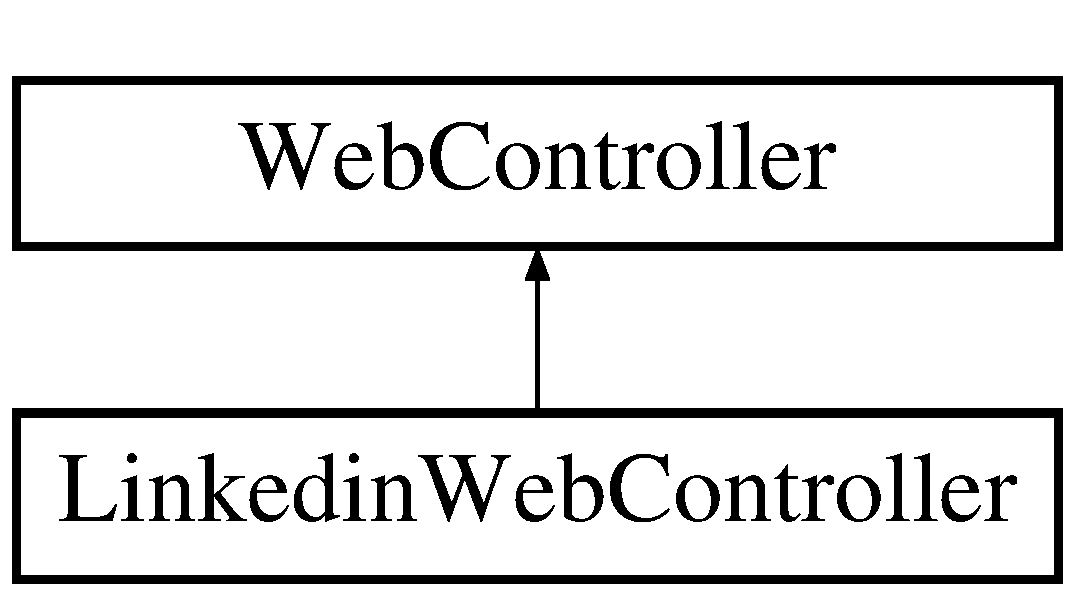
\includegraphics[height=2.000000cm]{classLinkedinWebController}
\end{center}
\end{figure}
\subsection*{Métodos públicos}
\begin{DoxyCompactItemize}
\item 
\hyperlink{classLinkedinWebController_a68424eeecce77f91b7e2a9f34928fde0}{Linkedin\+Web\+Controller} ()
\item 
\hyperlink{classLinkedinWebController_a9f795c0874b74594b8434317e2795e9a}{$\sim$\+Linkedin\+Web\+Controller} ()
\item 
virtual void \hyperlink{classLinkedinWebController_aa685544945b192b9149deaba1304f33b}{setup} ()
\item 
void \hyperlink{classLinkedinWebController_af300383547b94080bc7edbee9624b852}{hello} (Mongoose\+::\+Request \&request, Mongoose\+::\+Stream\+Response \&response)
\item 
void \hyperlink{classLinkedinWebController_a56c448409227ffb804019899ff5d4488}{form} (Mongoose\+::\+Request \&request, Mongoose\+::\+Stream\+Response \&response)
\item 
void \hyperlink{classLinkedinWebController_a20cc880e30969f5626f6553c6182a78f}{form\+Post} (Mongoose\+::\+Request \&request, Mongoose\+::\+Stream\+Response \&response)
\item 
void \hyperlink{classLinkedinWebController_acdbbbe5c9139f0f7959ca70df699c255}{session} (Mongoose\+::\+Request \&request, Mongoose\+::\+Stream\+Response \&response)
\item 
void \hyperlink{classLinkedinWebController_a44ae4397ca88552b07b6bc8e57c713fc}{forbid} (Mongoose\+::\+Request \&request, Mongoose\+::\+Stream\+Response \&response)
\item 
void \hyperlink{classLinkedinWebController_abe96bf2fa8e3084d45b34dda30331171}{exception} (Mongoose\+::\+Request \&request, Mongoose\+::\+Stream\+Response \&response)
\item 
void \hyperlink{classLinkedinWebController_a380a3e6b865576901e066b82a7279460}{upload\+Form} (Mongoose\+::\+Request \&request, Mongoose\+::\+Stream\+Response \&response)
\item 
void \hyperlink{classLinkedinWebController_a8cd6c4499d69595ddc6c349fa31c2c28}{upload} (Mongoose\+::\+Request \&request, Mongoose\+::\+Stream\+Response \&response)
\end{DoxyCompactItemize}


\subsection{Documentación del constructor y destructor}
\mbox{\Hypertarget{classLinkedinWebController_a68424eeecce77f91b7e2a9f34928fde0}\label{classLinkedinWebController_a68424eeecce77f91b7e2a9f34928fde0}} 
\index{Linkedin\+Web\+Controller@{Linkedin\+Web\+Controller}!Linkedin\+Web\+Controller@{Linkedin\+Web\+Controller}}
\index{Linkedin\+Web\+Controller@{Linkedin\+Web\+Controller}!Linkedin\+Web\+Controller@{Linkedin\+Web\+Controller}}
\subsubsection{\texorpdfstring{Linkedin\+Web\+Controller()}{LinkedinWebController()}}
{\footnotesize\ttfamily Linkedin\+Web\+Controller\+::\+Linkedin\+Web\+Controller (\begin{DoxyParamCaption}{ }\end{DoxyParamCaption})}

\mbox{\Hypertarget{classLinkedinWebController_a9f795c0874b74594b8434317e2795e9a}\label{classLinkedinWebController_a9f795c0874b74594b8434317e2795e9a}} 
\index{Linkedin\+Web\+Controller@{Linkedin\+Web\+Controller}!````~Linkedin\+Web\+Controller@{$\sim$\+Linkedin\+Web\+Controller}}
\index{````~Linkedin\+Web\+Controller@{$\sim$\+Linkedin\+Web\+Controller}!Linkedin\+Web\+Controller@{Linkedin\+Web\+Controller}}
\subsubsection{\texorpdfstring{$\sim$\+Linkedin\+Web\+Controller()}{~LinkedinWebController()}}
{\footnotesize\ttfamily Linkedin\+Web\+Controller\+::$\sim$\+Linkedin\+Web\+Controller (\begin{DoxyParamCaption}{ }\end{DoxyParamCaption})}



\subsection{Documentación de las funciones miembro}
\mbox{\Hypertarget{classLinkedinWebController_abe96bf2fa8e3084d45b34dda30331171}\label{classLinkedinWebController_abe96bf2fa8e3084d45b34dda30331171}} 
\index{Linkedin\+Web\+Controller@{Linkedin\+Web\+Controller}!exception@{exception}}
\index{exception@{exception}!Linkedin\+Web\+Controller@{Linkedin\+Web\+Controller}}
\subsubsection{\texorpdfstring{exception()}{exception()}}
{\footnotesize\ttfamily void Linkedin\+Web\+Controller\+::exception (\begin{DoxyParamCaption}\item[{Mongoose\+::\+Request \&}]{request,  }\item[{Mongoose\+::\+Stream\+Response \&}]{response }\end{DoxyParamCaption})}

\mbox{\Hypertarget{classLinkedinWebController_a44ae4397ca88552b07b6bc8e57c713fc}\label{classLinkedinWebController_a44ae4397ca88552b07b6bc8e57c713fc}} 
\index{Linkedin\+Web\+Controller@{Linkedin\+Web\+Controller}!forbid@{forbid}}
\index{forbid@{forbid}!Linkedin\+Web\+Controller@{Linkedin\+Web\+Controller}}
\subsubsection{\texorpdfstring{forbid()}{forbid()}}
{\footnotesize\ttfamily void Linkedin\+Web\+Controller\+::forbid (\begin{DoxyParamCaption}\item[{Mongoose\+::\+Request \&}]{request,  }\item[{Mongoose\+::\+Stream\+Response \&}]{response }\end{DoxyParamCaption})}

\mbox{\Hypertarget{classLinkedinWebController_a56c448409227ffb804019899ff5d4488}\label{classLinkedinWebController_a56c448409227ffb804019899ff5d4488}} 
\index{Linkedin\+Web\+Controller@{Linkedin\+Web\+Controller}!form@{form}}
\index{form@{form}!Linkedin\+Web\+Controller@{Linkedin\+Web\+Controller}}
\subsubsection{\texorpdfstring{form()}{form()}}
{\footnotesize\ttfamily void Linkedin\+Web\+Controller\+::form (\begin{DoxyParamCaption}\item[{Mongoose\+::\+Request \&}]{request,  }\item[{Mongoose\+::\+Stream\+Response \&}]{response }\end{DoxyParamCaption})}

\mbox{\Hypertarget{classLinkedinWebController_a20cc880e30969f5626f6553c6182a78f}\label{classLinkedinWebController_a20cc880e30969f5626f6553c6182a78f}} 
\index{Linkedin\+Web\+Controller@{Linkedin\+Web\+Controller}!form\+Post@{form\+Post}}
\index{form\+Post@{form\+Post}!Linkedin\+Web\+Controller@{Linkedin\+Web\+Controller}}
\subsubsection{\texorpdfstring{form\+Post()}{formPost()}}
{\footnotesize\ttfamily void Linkedin\+Web\+Controller\+::form\+Post (\begin{DoxyParamCaption}\item[{Mongoose\+::\+Request \&}]{request,  }\item[{Mongoose\+::\+Stream\+Response \&}]{response }\end{DoxyParamCaption})}

\mbox{\Hypertarget{classLinkedinWebController_af300383547b94080bc7edbee9624b852}\label{classLinkedinWebController_af300383547b94080bc7edbee9624b852}} 
\index{Linkedin\+Web\+Controller@{Linkedin\+Web\+Controller}!hello@{hello}}
\index{hello@{hello}!Linkedin\+Web\+Controller@{Linkedin\+Web\+Controller}}
\subsubsection{\texorpdfstring{hello()}{hello()}}
{\footnotesize\ttfamily void Linkedin\+Web\+Controller\+::hello (\begin{DoxyParamCaption}\item[{Mongoose\+::\+Request \&}]{request,  }\item[{Mongoose\+::\+Stream\+Response \&}]{response }\end{DoxyParamCaption})}

\mbox{\Hypertarget{classLinkedinWebController_acdbbbe5c9139f0f7959ca70df699c255}\label{classLinkedinWebController_acdbbbe5c9139f0f7959ca70df699c255}} 
\index{Linkedin\+Web\+Controller@{Linkedin\+Web\+Controller}!session@{session}}
\index{session@{session}!Linkedin\+Web\+Controller@{Linkedin\+Web\+Controller}}
\subsubsection{\texorpdfstring{session()}{session()}}
{\footnotesize\ttfamily void Linkedin\+Web\+Controller\+::session (\begin{DoxyParamCaption}\item[{Mongoose\+::\+Request \&}]{request,  }\item[{Mongoose\+::\+Stream\+Response \&}]{response }\end{DoxyParamCaption})}

\mbox{\Hypertarget{classLinkedinWebController_aa685544945b192b9149deaba1304f33b}\label{classLinkedinWebController_aa685544945b192b9149deaba1304f33b}} 
\index{Linkedin\+Web\+Controller@{Linkedin\+Web\+Controller}!setup@{setup}}
\index{setup@{setup}!Linkedin\+Web\+Controller@{Linkedin\+Web\+Controller}}
\subsubsection{\texorpdfstring{setup()}{setup()}}
{\footnotesize\ttfamily void Linkedin\+Web\+Controller\+::setup (\begin{DoxyParamCaption}{ }\end{DoxyParamCaption})\hspace{0.3cm}{\ttfamily [virtual]}}

\mbox{\Hypertarget{classLinkedinWebController_a8cd6c4499d69595ddc6c349fa31c2c28}\label{classLinkedinWebController_a8cd6c4499d69595ddc6c349fa31c2c28}} 
\index{Linkedin\+Web\+Controller@{Linkedin\+Web\+Controller}!upload@{upload}}
\index{upload@{upload}!Linkedin\+Web\+Controller@{Linkedin\+Web\+Controller}}
\subsubsection{\texorpdfstring{upload()}{upload()}}
{\footnotesize\ttfamily void Linkedin\+Web\+Controller\+::upload (\begin{DoxyParamCaption}\item[{Mongoose\+::\+Request \&}]{request,  }\item[{Mongoose\+::\+Stream\+Response \&}]{response }\end{DoxyParamCaption})}

\mbox{\Hypertarget{classLinkedinWebController_a380a3e6b865576901e066b82a7279460}\label{classLinkedinWebController_a380a3e6b865576901e066b82a7279460}} 
\index{Linkedin\+Web\+Controller@{Linkedin\+Web\+Controller}!upload\+Form@{upload\+Form}}
\index{upload\+Form@{upload\+Form}!Linkedin\+Web\+Controller@{Linkedin\+Web\+Controller}}
\subsubsection{\texorpdfstring{upload\+Form()}{uploadForm()}}
{\footnotesize\ttfamily void Linkedin\+Web\+Controller\+::upload\+Form (\begin{DoxyParamCaption}\item[{Mongoose\+::\+Request \&}]{request,  }\item[{Mongoose\+::\+Stream\+Response \&}]{response }\end{DoxyParamCaption})}



La documentación para esta clase fue generada a partir de los siguientes ficheros\+:\begin{DoxyCompactItemize}
\item 
/home/ezequiel/taller2/taller2/server/src/\hyperlink{LinkedinWebController_8h}{Linkedin\+Web\+Controller.\+h}\item 
/home/ezequiel/taller2/taller2/server/src/\hyperlink{LinkedinWebController_8cpp}{Linkedin\+Web\+Controller.\+cpp}\end{DoxyCompactItemize}

\hypertarget{classLog}{}\section{Referencia de la Clase Log}
\label{classLog}\index{Log@{Log}}


{\ttfamily \#include $<$log.\+h$>$}

\subsection*{Métodos públicos}
\begin{DoxyCompactItemize}
\item 
\hyperlink{classLog_a0fbfda88fbee5027c89f6eb121059360}{$\sim$\+Log} ()
\item 
void \hyperlink{classLog_ac659fa24adce6d3ed79be5c6ab4248ca}{log\+\_\+warning} (const std\+::string \&menssage)
\item 
void \hyperlink{classLog_a336032c9a87f2a6b0a463db7e2f7d1a4}{log\+\_\+error} (const std\+::string \&menssage)
\item 
void \hyperlink{classLog_a9af02d242cf75e658899c67ad9136fd7}{log\+\_\+info} (const std\+::string \&menssage)
\item 
void \hyperlink{classLog_a7ed913c04040b6ff20da0bd7306b92cd}{log\+\_\+debug} (const std\+::string \&menssage)
\end{DoxyCompactItemize}
\subsection*{Métodos públicos estáticos}
\begin{DoxyCompactItemize}
\item 
static \hyperlink{classLog}{Log} $\ast$ \hyperlink{classLog_a5046d929af7ff9a206279f2cd9e9d8e8}{get\+\_\+instance} ()
\end{DoxyCompactItemize}


\subsection{Documentación del constructor y destructor}
\mbox{\Hypertarget{classLog_a0fbfda88fbee5027c89f6eb121059360}\label{classLog_a0fbfda88fbee5027c89f6eb121059360}} 
\index{Log@{Log}!````~Log@{$\sim$\+Log}}
\index{````~Log@{$\sim$\+Log}!Log@{Log}}
\subsubsection{\texorpdfstring{$\sim$\+Log()}{~Log()}}
{\footnotesize\ttfamily Log\+::$\sim$\+Log (\begin{DoxyParamCaption}{ }\end{DoxyParamCaption})}



\subsection{Documentación de las funciones miembro}
\mbox{\Hypertarget{classLog_a5046d929af7ff9a206279f2cd9e9d8e8}\label{classLog_a5046d929af7ff9a206279f2cd9e9d8e8}} 
\index{Log@{Log}!get\+\_\+instance@{get\+\_\+instance}}
\index{get\+\_\+instance@{get\+\_\+instance}!Log@{Log}}
\subsubsection{\texorpdfstring{get\+\_\+instance()}{get\_instance()}}
{\footnotesize\ttfamily \hyperlink{classLog}{Log} $\ast$ Log\+::get\+\_\+instance (\begin{DoxyParamCaption}{ }\end{DoxyParamCaption})\hspace{0.3cm}{\ttfamily [static]}}

\mbox{\Hypertarget{classLog_a7ed913c04040b6ff20da0bd7306b92cd}\label{classLog_a7ed913c04040b6ff20da0bd7306b92cd}} 
\index{Log@{Log}!log\+\_\+debug@{log\+\_\+debug}}
\index{log\+\_\+debug@{log\+\_\+debug}!Log@{Log}}
\subsubsection{\texorpdfstring{log\+\_\+debug()}{log\_debug()}}
{\footnotesize\ttfamily void Log\+::log\+\_\+debug (\begin{DoxyParamCaption}\item[{const std\+::string \&}]{menssage }\end{DoxyParamCaption})}

\mbox{\Hypertarget{classLog_a336032c9a87f2a6b0a463db7e2f7d1a4}\label{classLog_a336032c9a87f2a6b0a463db7e2f7d1a4}} 
\index{Log@{Log}!log\+\_\+error@{log\+\_\+error}}
\index{log\+\_\+error@{log\+\_\+error}!Log@{Log}}
\subsubsection{\texorpdfstring{log\+\_\+error()}{log\_error()}}
{\footnotesize\ttfamily void Log\+::log\+\_\+error (\begin{DoxyParamCaption}\item[{const std\+::string \&}]{menssage }\end{DoxyParamCaption})}

\mbox{\Hypertarget{classLog_a9af02d242cf75e658899c67ad9136fd7}\label{classLog_a9af02d242cf75e658899c67ad9136fd7}} 
\index{Log@{Log}!log\+\_\+info@{log\+\_\+info}}
\index{log\+\_\+info@{log\+\_\+info}!Log@{Log}}
\subsubsection{\texorpdfstring{log\+\_\+info()}{log\_info()}}
{\footnotesize\ttfamily void Log\+::log\+\_\+info (\begin{DoxyParamCaption}\item[{const std\+::string \&}]{menssage }\end{DoxyParamCaption})}

\mbox{\Hypertarget{classLog_ac659fa24adce6d3ed79be5c6ab4248ca}\label{classLog_ac659fa24adce6d3ed79be5c6ab4248ca}} 
\index{Log@{Log}!log\+\_\+warning@{log\+\_\+warning}}
\index{log\+\_\+warning@{log\+\_\+warning}!Log@{Log}}
\subsubsection{\texorpdfstring{log\+\_\+warning()}{log\_warning()}}
{\footnotesize\ttfamily void Log\+::log\+\_\+warning (\begin{DoxyParamCaption}\item[{const std\+::string \&}]{menssage }\end{DoxyParamCaption})}



La documentación para esta clase fue generada a partir de los siguientes ficheros\+:\begin{DoxyCompactItemize}
\item 
/home/ezequiel/taller2/taller2/server/src/\hyperlink{log_8h}{log.\+h}\item 
/home/ezequiel/taller2/taller2/server/src/\hyperlink{log_8cpp}{log.\+cpp}\end{DoxyCompactItemize}

\hypertarget{classMD5}{}\section{Referencia de la Clase M\+D5}
\label{classMD5}\index{M\+D5@{M\+D5}}


{\ttfamily \#include $<$md5.\+h$>$}

\subsection*{Tipos públicos}
\begin{DoxyCompactItemize}
\item 
typedef unsigned int \hyperlink{classMD5_aa836972700679dbcff6ae8337f6db464}{size\+\_\+type}
\end{DoxyCompactItemize}
\subsection*{Métodos públicos}
\begin{DoxyCompactItemize}
\item 
\hyperlink{classMD5_afa6155ec36de415ab2dcf5e54b670d13}{M\+D5} ()
\item 
\hyperlink{classMD5_a155356ffd713345e69e6dcbd9f8da6ce}{M\+D5} (const std\+::string \&text)
\item 
void \hyperlink{classMD5_ac5ddf6cd8f940422396d321ea90ed045}{update} (const unsigned char $\ast$buf, \hyperlink{classMD5_aa836972700679dbcff6ae8337f6db464}{size\+\_\+type} length)
\item 
void \hyperlink{classMD5_ac5ccba375539b993958fb235f8ac849c}{update} (const char $\ast$buf, \hyperlink{classMD5_aa836972700679dbcff6ae8337f6db464}{size\+\_\+type} length)
\item 
\hyperlink{classMD5}{M\+D5} \& \hyperlink{classMD5_a10f607494a3f2e3e515fc4b99d1a06cc}{finalize} ()
\item 
std\+::string \hyperlink{classMD5_aaf466f683b4bd8b1b66544f48bf09608}{hexdigest} () const
\end{DoxyCompactItemize}
\subsection*{Amigas}
\begin{DoxyCompactItemize}
\item 
std\+::ostream \& \hyperlink{classMD5_a0739666fd0f3a7117546f6c50e0783b2}{operator$<$$<$} (std\+::ostream \&, \hyperlink{classMD5}{M\+D5} \hyperlink{md5_8h_a92c6eed2e9b51298af559aff6792770b}{md5})
\end{DoxyCompactItemize}


\subsection{Documentación de los \textquotesingle{}Typedef\textquotesingle{} miembros de la clase}
\mbox{\Hypertarget{classMD5_aa836972700679dbcff6ae8337f6db464}\label{classMD5_aa836972700679dbcff6ae8337f6db464}} 
\index{M\+D5@{M\+D5}!size\+\_\+type@{size\+\_\+type}}
\index{size\+\_\+type@{size\+\_\+type}!M\+D5@{M\+D5}}
\subsubsection{\texorpdfstring{size\+\_\+type}{size\_type}}
{\footnotesize\ttfamily typedef unsigned int \hyperlink{classMD5_aa836972700679dbcff6ae8337f6db464}{M\+D5\+::size\+\_\+type}}



\subsection{Documentación del constructor y destructor}
\mbox{\Hypertarget{classMD5_afa6155ec36de415ab2dcf5e54b670d13}\label{classMD5_afa6155ec36de415ab2dcf5e54b670d13}} 
\index{M\+D5@{M\+D5}!M\+D5@{M\+D5}}
\index{M\+D5@{M\+D5}!M\+D5@{M\+D5}}
\subsubsection{\texorpdfstring{M\+D5()}{MD5()}\hspace{0.1cm}{\footnotesize\ttfamily [1/2]}}
{\footnotesize\ttfamily M\+D5\+::\+M\+D5 (\begin{DoxyParamCaption}{ }\end{DoxyParamCaption})}

\mbox{\Hypertarget{classMD5_a155356ffd713345e69e6dcbd9f8da6ce}\label{classMD5_a155356ffd713345e69e6dcbd9f8da6ce}} 
\index{M\+D5@{M\+D5}!M\+D5@{M\+D5}}
\index{M\+D5@{M\+D5}!M\+D5@{M\+D5}}
\subsubsection{\texorpdfstring{M\+D5()}{MD5()}\hspace{0.1cm}{\footnotesize\ttfamily [2/2]}}
{\footnotesize\ttfamily M\+D5\+::\+M\+D5 (\begin{DoxyParamCaption}\item[{const std\+::string \&}]{text }\end{DoxyParamCaption})}



\subsection{Documentación de las funciones miembro}
\mbox{\Hypertarget{classMD5_a10f607494a3f2e3e515fc4b99d1a06cc}\label{classMD5_a10f607494a3f2e3e515fc4b99d1a06cc}} 
\index{M\+D5@{M\+D5}!finalize@{finalize}}
\index{finalize@{finalize}!M\+D5@{M\+D5}}
\subsubsection{\texorpdfstring{finalize()}{finalize()}}
{\footnotesize\ttfamily \hyperlink{classMD5}{M\+D5} \& M\+D5\+::finalize (\begin{DoxyParamCaption}{ }\end{DoxyParamCaption})}

\mbox{\Hypertarget{classMD5_aaf466f683b4bd8b1b66544f48bf09608}\label{classMD5_aaf466f683b4bd8b1b66544f48bf09608}} 
\index{M\+D5@{M\+D5}!hexdigest@{hexdigest}}
\index{hexdigest@{hexdigest}!M\+D5@{M\+D5}}
\subsubsection{\texorpdfstring{hexdigest()}{hexdigest()}}
{\footnotesize\ttfamily std\+::string M\+D5\+::hexdigest (\begin{DoxyParamCaption}{ }\end{DoxyParamCaption}) const}

\mbox{\Hypertarget{classMD5_ac5ddf6cd8f940422396d321ea90ed045}\label{classMD5_ac5ddf6cd8f940422396d321ea90ed045}} 
\index{M\+D5@{M\+D5}!update@{update}}
\index{update@{update}!M\+D5@{M\+D5}}
\subsubsection{\texorpdfstring{update()}{update()}\hspace{0.1cm}{\footnotesize\ttfamily [1/2]}}
{\footnotesize\ttfamily void M\+D5\+::update (\begin{DoxyParamCaption}\item[{const unsigned char $\ast$}]{buf,  }\item[{\hyperlink{classMD5_aa836972700679dbcff6ae8337f6db464}{size\+\_\+type}}]{length }\end{DoxyParamCaption})}

\mbox{\Hypertarget{classMD5_ac5ccba375539b993958fb235f8ac849c}\label{classMD5_ac5ccba375539b993958fb235f8ac849c}} 
\index{M\+D5@{M\+D5}!update@{update}}
\index{update@{update}!M\+D5@{M\+D5}}
\subsubsection{\texorpdfstring{update()}{update()}\hspace{0.1cm}{\footnotesize\ttfamily [2/2]}}
{\footnotesize\ttfamily void M\+D5\+::update (\begin{DoxyParamCaption}\item[{const char $\ast$}]{buf,  }\item[{\hyperlink{classMD5_aa836972700679dbcff6ae8337f6db464}{size\+\_\+type}}]{length }\end{DoxyParamCaption})}



\subsection{Documentación de las funciones relacionadas y clases amigas}
\mbox{\Hypertarget{classMD5_a0739666fd0f3a7117546f6c50e0783b2}\label{classMD5_a0739666fd0f3a7117546f6c50e0783b2}} 
\index{M\+D5@{M\+D5}!operator$<$$<$@{operator$<$$<$}}
\index{operator$<$$<$@{operator$<$$<$}!M\+D5@{M\+D5}}
\subsubsection{\texorpdfstring{operator$<$$<$}{operator<<}}
{\footnotesize\ttfamily std\+::ostream\& operator$<$$<$ (\begin{DoxyParamCaption}\item[{std\+::ostream \&}]{out,  }\item[{\hyperlink{classMD5}{M\+D5}}]{md5 }\end{DoxyParamCaption})\hspace{0.3cm}{\ttfamily [friend]}}



La documentación para esta clase fue generada a partir de los siguientes ficheros\+:\begin{DoxyCompactItemize}
\item 
/home/ezequiel/taller2/taller2/server/src/\hyperlink{md5_8h}{md5.\+h}\item 
/home/ezequiel/taller2/taller2/server/src/\hyperlink{md5_8cpp}{md5.\+cpp}\end{DoxyCompactItemize}

\hypertarget{structOrderByVotes}{}\section{Referencia de la Estructura Order\+By\+Votes}
\label{structOrderByVotes}\index{Order\+By\+Votes@{Order\+By\+Votes}}


{\ttfamily \#include $<$User\+Handler.\+h$>$}

\subsection*{Métodos públicos}
\begin{DoxyCompactItemize}
\item 
bool \hyperlink{structOrderByVotes_af43d1fded49999b848b8b1040fa56533}{operator()} (\hyperlink{classUser}{User} const \&a, \hyperlink{classUser}{User} const \&b)
\end{DoxyCompactItemize}


\subsection{Documentación de las funciones miembro}
\mbox{\Hypertarget{structOrderByVotes_af43d1fded49999b848b8b1040fa56533}\label{structOrderByVotes_af43d1fded49999b848b8b1040fa56533}} 
\index{Order\+By\+Votes@{Order\+By\+Votes}!operator()@{operator()}}
\index{operator()@{operator()}!Order\+By\+Votes@{Order\+By\+Votes}}
\subsubsection{\texorpdfstring{operator()()}{operator()()}}
{\footnotesize\ttfamily bool Order\+By\+Votes\+::operator() (\begin{DoxyParamCaption}\item[{\hyperlink{classUser}{User} const \&}]{a,  }\item[{\hyperlink{classUser}{User} const \&}]{b }\end{DoxyParamCaption})\hspace{0.3cm}{\ttfamily [inline]}}



La documentación para esta estructura fue generada a partir del siguiente fichero\+:\begin{DoxyCompactItemize}
\item 
/home/ezequiel/taller2/taller2/server/src/\hyperlink{UserHandler_8h}{User\+Handler.\+h}\end{DoxyCompactItemize}

\hypertarget{classUser}{}\section{Referencia de la Clase User}
\label{classUser}\index{User@{User}}


{\ttfamily \#include $<$User.\+h$>$}

\subsection*{Métodos públicos}
\begin{DoxyCompactItemize}
\item 
\hyperlink{classUser_a39b6626888c80680166832d96a8ac4c7}{User} (std\+::string json\+\_\+value)
\item 
\hyperlink{classUser_a4a0137053e591fbb79d9057dd7d2283d}{User} ()
\item 
\hyperlink{classUser_ac00b72ad64eb4149f7b21b9f5468c2b2}{$\sim$\+User} ()
\item 
std\+::string \hyperlink{classUser_a3394f9749a9e0c807ff34d148d9f835a}{serialize} ()
\item 
std\+::string \hyperlink{classUser_a027b5483be61adf2d2b18c06e0f76409}{database\+\_\+serialize} ()
\item 
std\+::string \hyperlink{classUser_ac140c8f3831f0c137a0356b5c5d1ac0c}{id} () const
\item 
std\+::string \hyperlink{classUser_afced0a5a8d577143c88f9ec8d36e0510}{get\+\_\+email} ()
\item 
std\+::string \hyperlink{classUser_a86c6040cbc76ac12c7f154b054bd1035}{get\+\_\+name} ()
\item 
std\+::string \hyperlink{classUser_a6f128d38b5cf38e1345b109f7264624f}{get\+\_\+dob} ()
\item 
std\+::string \hyperlink{classUser_a0b1c6d729cb6260557efcc614019ad3d}{get\+\_\+city} ()
\item 
std\+::string \hyperlink{classUser_abd12a463644dad79711a99e9b4ca5f81}{get\+\_\+summary} ()
\item 
std\+::string \hyperlink{classUser_aca8fcd8329ceba292fc4b762962f514a}{get\+\_\+profile\+\_\+photo} ()
\item 
void \hyperlink{classUser_afe3e0fa5e2a7189e2ec94cb126cb1ee0}{replace\+\_\+not\+\_\+null} (std\+::string field, std\+::string value)
\item 
void \hyperlink{classUser_a4452f9cee8e5928ca3feb248ddf61ed5}{send\+\_\+request} (\hyperlink{classUser}{User} \&other\+\_\+user)
\item 
int \hyperlink{classUser_aa165982b75d55551626758b6fffac803}{requests} ()
\item 
void \hyperlink{classUser_aecb82a4b3775064eb10fcdaf288fbfa4}{accept\+\_\+request} (\hyperlink{classUser}{User} \&other\+\_\+user)
\item 
void \hyperlink{classUser_a6b431d3face2db990dcdf48d74e745d6}{reject\+\_\+request} (\hyperlink{classUser}{User} \&other\+\_\+user)
\item 
std\+::list$<$ std\+::string $>$ \hyperlink{classUser_a4d4864c9959ed4db8c1e92ab924f0d76}{friends} ()
\item 
void \hyperlink{classUser_ae7bca2cb41eac8d576a781ac2de1b150}{vote\+\_\+for} (\hyperlink{classUser}{User} \&other\+\_\+user)
\item 
size\+\_\+t \hyperlink{classUser_a0b8e3871b4c9623b37dcfed43ddee1b3}{votes} () const
\item 
bool \hyperlink{classUser_a29b6fe2813703559ecb60f2f5614302f}{was\+\_\+voted\+\_\+by} (const \hyperlink{classUser}{User} \&other\+\_\+user)
\end{DoxyCompactItemize}


\subsection{Documentación del constructor y destructor}
\mbox{\Hypertarget{classUser_a39b6626888c80680166832d96a8ac4c7}\label{classUser_a39b6626888c80680166832d96a8ac4c7}} 
\index{User@{User}!User@{User}}
\index{User@{User}!User@{User}}
\subsubsection{\texorpdfstring{User()}{User()}\hspace{0.1cm}{\footnotesize\ttfamily [1/2]}}
{\footnotesize\ttfamily User\+::\+User (\begin{DoxyParamCaption}\item[{std\+::string}]{json\+\_\+value }\end{DoxyParamCaption})}

\mbox{\Hypertarget{classUser_a4a0137053e591fbb79d9057dd7d2283d}\label{classUser_a4a0137053e591fbb79d9057dd7d2283d}} 
\index{User@{User}!User@{User}}
\index{User@{User}!User@{User}}
\subsubsection{\texorpdfstring{User()}{User()}\hspace{0.1cm}{\footnotesize\ttfamily [2/2]}}
{\footnotesize\ttfamily User\+::\+User (\begin{DoxyParamCaption}{ }\end{DoxyParamCaption})}

\mbox{\Hypertarget{classUser_ac00b72ad64eb4149f7b21b9f5468c2b2}\label{classUser_ac00b72ad64eb4149f7b21b9f5468c2b2}} 
\index{User@{User}!````~User@{$\sim$\+User}}
\index{````~User@{$\sim$\+User}!User@{User}}
\subsubsection{\texorpdfstring{$\sim$\+User()}{~User()}}
{\footnotesize\ttfamily User\+::$\sim$\+User (\begin{DoxyParamCaption}{ }\end{DoxyParamCaption})}



\subsection{Documentación de las funciones miembro}
\mbox{\Hypertarget{classUser_aecb82a4b3775064eb10fcdaf288fbfa4}\label{classUser_aecb82a4b3775064eb10fcdaf288fbfa4}} 
\index{User@{User}!accept\+\_\+request@{accept\+\_\+request}}
\index{accept\+\_\+request@{accept\+\_\+request}!User@{User}}
\subsubsection{\texorpdfstring{accept\+\_\+request()}{accept\_request()}}
{\footnotesize\ttfamily void User\+::accept\+\_\+request (\begin{DoxyParamCaption}\item[{\hyperlink{classUser}{User} \&}]{other\+\_\+user }\end{DoxyParamCaption})}

\mbox{\Hypertarget{classUser_a027b5483be61adf2d2b18c06e0f76409}\label{classUser_a027b5483be61adf2d2b18c06e0f76409}} 
\index{User@{User}!database\+\_\+serialize@{database\+\_\+serialize}}
\index{database\+\_\+serialize@{database\+\_\+serialize}!User@{User}}
\subsubsection{\texorpdfstring{database\+\_\+serialize()}{database\_serialize()}}
{\footnotesize\ttfamily std\+::string User\+::database\+\_\+serialize (\begin{DoxyParamCaption}{ }\end{DoxyParamCaption})}

\mbox{\Hypertarget{classUser_a4d4864c9959ed4db8c1e92ab924f0d76}\label{classUser_a4d4864c9959ed4db8c1e92ab924f0d76}} 
\index{User@{User}!friends@{friends}}
\index{friends@{friends}!User@{User}}
\subsubsection{\texorpdfstring{friends()}{friends()}}
{\footnotesize\ttfamily std\+::list$<$ std\+::string $>$ User\+::friends (\begin{DoxyParamCaption}{ }\end{DoxyParamCaption})}

\mbox{\Hypertarget{classUser_a0b1c6d729cb6260557efcc614019ad3d}\label{classUser_a0b1c6d729cb6260557efcc614019ad3d}} 
\index{User@{User}!get\+\_\+city@{get\+\_\+city}}
\index{get\+\_\+city@{get\+\_\+city}!User@{User}}
\subsubsection{\texorpdfstring{get\+\_\+city()}{get\_city()}}
{\footnotesize\ttfamily std\+::string User\+::get\+\_\+city (\begin{DoxyParamCaption}{ }\end{DoxyParamCaption})}

\mbox{\Hypertarget{classUser_a6f128d38b5cf38e1345b109f7264624f}\label{classUser_a6f128d38b5cf38e1345b109f7264624f}} 
\index{User@{User}!get\+\_\+dob@{get\+\_\+dob}}
\index{get\+\_\+dob@{get\+\_\+dob}!User@{User}}
\subsubsection{\texorpdfstring{get\+\_\+dob()}{get\_dob()}}
{\footnotesize\ttfamily std\+::string User\+::get\+\_\+dob (\begin{DoxyParamCaption}{ }\end{DoxyParamCaption})}

\mbox{\Hypertarget{classUser_afced0a5a8d577143c88f9ec8d36e0510}\label{classUser_afced0a5a8d577143c88f9ec8d36e0510}} 
\index{User@{User}!get\+\_\+email@{get\+\_\+email}}
\index{get\+\_\+email@{get\+\_\+email}!User@{User}}
\subsubsection{\texorpdfstring{get\+\_\+email()}{get\_email()}}
{\footnotesize\ttfamily std\+::string User\+::get\+\_\+email (\begin{DoxyParamCaption}{ }\end{DoxyParamCaption})}

\mbox{\Hypertarget{classUser_a86c6040cbc76ac12c7f154b054bd1035}\label{classUser_a86c6040cbc76ac12c7f154b054bd1035}} 
\index{User@{User}!get\+\_\+name@{get\+\_\+name}}
\index{get\+\_\+name@{get\+\_\+name}!User@{User}}
\subsubsection{\texorpdfstring{get\+\_\+name()}{get\_name()}}
{\footnotesize\ttfamily std\+::string User\+::get\+\_\+name (\begin{DoxyParamCaption}{ }\end{DoxyParamCaption})}

\mbox{\Hypertarget{classUser_aca8fcd8329ceba292fc4b762962f514a}\label{classUser_aca8fcd8329ceba292fc4b762962f514a}} 
\index{User@{User}!get\+\_\+profile\+\_\+photo@{get\+\_\+profile\+\_\+photo}}
\index{get\+\_\+profile\+\_\+photo@{get\+\_\+profile\+\_\+photo}!User@{User}}
\subsubsection{\texorpdfstring{get\+\_\+profile\+\_\+photo()}{get\_profile\_photo()}}
{\footnotesize\ttfamily std\+::string User\+::get\+\_\+profile\+\_\+photo (\begin{DoxyParamCaption}{ }\end{DoxyParamCaption})}

\mbox{\Hypertarget{classUser_abd12a463644dad79711a99e9b4ca5f81}\label{classUser_abd12a463644dad79711a99e9b4ca5f81}} 
\index{User@{User}!get\+\_\+summary@{get\+\_\+summary}}
\index{get\+\_\+summary@{get\+\_\+summary}!User@{User}}
\subsubsection{\texorpdfstring{get\+\_\+summary()}{get\_summary()}}
{\footnotesize\ttfamily std\+::string User\+::get\+\_\+summary (\begin{DoxyParamCaption}{ }\end{DoxyParamCaption})}

\mbox{\Hypertarget{classUser_ac140c8f3831f0c137a0356b5c5d1ac0c}\label{classUser_ac140c8f3831f0c137a0356b5c5d1ac0c}} 
\index{User@{User}!id@{id}}
\index{id@{id}!User@{User}}
\subsubsection{\texorpdfstring{id()}{id()}}
{\footnotesize\ttfamily std\+::string User\+::id (\begin{DoxyParamCaption}{ }\end{DoxyParamCaption}) const}

\mbox{\Hypertarget{classUser_a6b431d3face2db990dcdf48d74e745d6}\label{classUser_a6b431d3face2db990dcdf48d74e745d6}} 
\index{User@{User}!reject\+\_\+request@{reject\+\_\+request}}
\index{reject\+\_\+request@{reject\+\_\+request}!User@{User}}
\subsubsection{\texorpdfstring{reject\+\_\+request()}{reject\_request()}}
{\footnotesize\ttfamily void User\+::reject\+\_\+request (\begin{DoxyParamCaption}\item[{\hyperlink{classUser}{User} \&}]{other\+\_\+user }\end{DoxyParamCaption})}

\mbox{\Hypertarget{classUser_afe3e0fa5e2a7189e2ec94cb126cb1ee0}\label{classUser_afe3e0fa5e2a7189e2ec94cb126cb1ee0}} 
\index{User@{User}!replace\+\_\+not\+\_\+null@{replace\+\_\+not\+\_\+null}}
\index{replace\+\_\+not\+\_\+null@{replace\+\_\+not\+\_\+null}!User@{User}}
\subsubsection{\texorpdfstring{replace\+\_\+not\+\_\+null()}{replace\_not\_null()}}
{\footnotesize\ttfamily void User\+::replace\+\_\+not\+\_\+null (\begin{DoxyParamCaption}\item[{std\+::string}]{field,  }\item[{std\+::string}]{value }\end{DoxyParamCaption})}

\mbox{\Hypertarget{classUser_aa165982b75d55551626758b6fffac803}\label{classUser_aa165982b75d55551626758b6fffac803}} 
\index{User@{User}!requests@{requests}}
\index{requests@{requests}!User@{User}}
\subsubsection{\texorpdfstring{requests()}{requests()}}
{\footnotesize\ttfamily int User\+::requests (\begin{DoxyParamCaption}{ }\end{DoxyParamCaption})}

\mbox{\Hypertarget{classUser_a4452f9cee8e5928ca3feb248ddf61ed5}\label{classUser_a4452f9cee8e5928ca3feb248ddf61ed5}} 
\index{User@{User}!send\+\_\+request@{send\+\_\+request}}
\index{send\+\_\+request@{send\+\_\+request}!User@{User}}
\subsubsection{\texorpdfstring{send\+\_\+request()}{send\_request()}}
{\footnotesize\ttfamily void User\+::send\+\_\+request (\begin{DoxyParamCaption}\item[{\hyperlink{classUser}{User} \&}]{other\+\_\+user }\end{DoxyParamCaption})}

\mbox{\Hypertarget{classUser_a3394f9749a9e0c807ff34d148d9f835a}\label{classUser_a3394f9749a9e0c807ff34d148d9f835a}} 
\index{User@{User}!serialize@{serialize}}
\index{serialize@{serialize}!User@{User}}
\subsubsection{\texorpdfstring{serialize()}{serialize()}}
{\footnotesize\ttfamily std\+::string User\+::serialize (\begin{DoxyParamCaption}{ }\end{DoxyParamCaption})}

\mbox{\Hypertarget{classUser_ae7bca2cb41eac8d576a781ac2de1b150}\label{classUser_ae7bca2cb41eac8d576a781ac2de1b150}} 
\index{User@{User}!vote\+\_\+for@{vote\+\_\+for}}
\index{vote\+\_\+for@{vote\+\_\+for}!User@{User}}
\subsubsection{\texorpdfstring{vote\+\_\+for()}{vote\_for()}}
{\footnotesize\ttfamily void User\+::vote\+\_\+for (\begin{DoxyParamCaption}\item[{\hyperlink{classUser}{User} \&}]{other\+\_\+user }\end{DoxyParamCaption})}

\mbox{\Hypertarget{classUser_a0b8e3871b4c9623b37dcfed43ddee1b3}\label{classUser_a0b8e3871b4c9623b37dcfed43ddee1b3}} 
\index{User@{User}!votes@{votes}}
\index{votes@{votes}!User@{User}}
\subsubsection{\texorpdfstring{votes()}{votes()}}
{\footnotesize\ttfamily size\+\_\+t User\+::votes (\begin{DoxyParamCaption}{ }\end{DoxyParamCaption}) const}

\mbox{\Hypertarget{classUser_a29b6fe2813703559ecb60f2f5614302f}\label{classUser_a29b6fe2813703559ecb60f2f5614302f}} 
\index{User@{User}!was\+\_\+voted\+\_\+by@{was\+\_\+voted\+\_\+by}}
\index{was\+\_\+voted\+\_\+by@{was\+\_\+voted\+\_\+by}!User@{User}}
\subsubsection{\texorpdfstring{was\+\_\+voted\+\_\+by()}{was\_voted\_by()}}
{\footnotesize\ttfamily bool User\+::was\+\_\+voted\+\_\+by (\begin{DoxyParamCaption}\item[{const \hyperlink{classUser}{User} \&}]{other\+\_\+user }\end{DoxyParamCaption})}



La documentación para esta clase fue generada a partir de los siguientes ficheros\+:\begin{DoxyCompactItemize}
\item 
/home/ezequiel/taller2/taller2/server/src/\hyperlink{User_8h}{User.\+h}\item 
/home/ezequiel/taller2/taller2/server/src/\hyperlink{User_8cpp}{User.\+cpp}\end{DoxyCompactItemize}

\hypertarget{classUserHandler}{}\section{Referencia de la Clase User\+Handler}
\label{classUserHandler}\index{User\+Handler@{User\+Handler}}


{\ttfamily \#include $<$User\+Handler.\+h$>$}

\subsection*{Métodos públicos}
\begin{DoxyCompactItemize}
\item 
bool \hyperlink{classUserHandler_ad07770b45bee5c2e42059a712fa8dd03}{user\+\_\+exists} (std\+::string user\+\_\+name)
\item 
void \hyperlink{classUserHandler_a24a57bdf7dbc66654b2b87059474af3f}{create\+\_\+user} (std\+::string fb\+\_\+id)
\item 
\hyperlink{classUser}{User} \hyperlink{classUserHandler_a89c1cf91efd6184a41368cdbd59f7908}{get\+\_\+user} (std\+::string user\+\_\+name)
\item 
void \hyperlink{classUserHandler_a54f7a36d48a334c7f5cc176f5f0c00ef}{save\+\_\+user} (\hyperlink{classUser}{User} \&user)
\item 
std\+::map$<$ std\+::string, std\+::string $>$ \hyperlink{classUserHandler_a970aeeb9a856f5413a0759f26d540a93}{lookup} (std\+::string query)
\item 
void \hyperlink{classUserHandler_ad687e0e4c993e40586c829dd18a8bd37}{send\+\_\+request} (std\+::string from\+\_\+user, std\+::string to\+\_\+user)
\item 
void \hyperlink{classUserHandler_aed1b8c59e28db3653dfae14721308c7e}{answer\+\_\+request} (std\+::string from\+\_\+user, std\+::string to\+\_\+user, bool accept)
\item 
std\+::map$<$ std\+::string, std\+::string $>$ \hyperlink{classUserHandler_a37abd677dead8a0c023a760c80e32d88}{get\+\_\+friends} (std\+::string user\+\_\+id)
\item 
void \hyperlink{classUserHandler_a0d5cc1c26560cd14e4f1a9bcf22db18a}{user\+\_\+vote} (std\+::string from\+\_\+user, std\+::string voted\+\_\+user)
\item 
\hyperlink{UserHandler_8h_a8dd774344f3a2ec6200ac8cbdfd3bf1c}{vote\+\_\+queue} \hyperlink{classUserHandler_a4c2cc3fcbff935b81746d2d3a77006b8}{most\+\_\+popular} ()
\end{DoxyCompactItemize}
\subsection*{Métodos públicos estáticos}
\begin{DoxyCompactItemize}
\item 
static \hyperlink{classUserHandler}{User\+Handler} \& \hyperlink{classUserHandler_ac4f67acbcfe4262169243a11f677a337}{get\+\_\+instance} ()
\end{DoxyCompactItemize}


\subsection{Documentación de las funciones miembro}
\mbox{\Hypertarget{classUserHandler_aed1b8c59e28db3653dfae14721308c7e}\label{classUserHandler_aed1b8c59e28db3653dfae14721308c7e}} 
\index{User\+Handler@{User\+Handler}!answer\+\_\+request@{answer\+\_\+request}}
\index{answer\+\_\+request@{answer\+\_\+request}!User\+Handler@{User\+Handler}}
\subsubsection{\texorpdfstring{answer\+\_\+request()}{answer\_request()}}
{\footnotesize\ttfamily void User\+Handler\+::answer\+\_\+request (\begin{DoxyParamCaption}\item[{std\+::string}]{from\+\_\+user,  }\item[{std\+::string}]{to\+\_\+user,  }\item[{bool}]{accept }\end{DoxyParamCaption})}

\mbox{\Hypertarget{classUserHandler_a24a57bdf7dbc66654b2b87059474af3f}\label{classUserHandler_a24a57bdf7dbc66654b2b87059474af3f}} 
\index{User\+Handler@{User\+Handler}!create\+\_\+user@{create\+\_\+user}}
\index{create\+\_\+user@{create\+\_\+user}!User\+Handler@{User\+Handler}}
\subsubsection{\texorpdfstring{create\+\_\+user()}{create\_user()}}
{\footnotesize\ttfamily void User\+Handler\+::create\+\_\+user (\begin{DoxyParamCaption}\item[{std\+::string}]{fb\+\_\+id }\end{DoxyParamCaption})}

\mbox{\Hypertarget{classUserHandler_a37abd677dead8a0c023a760c80e32d88}\label{classUserHandler_a37abd677dead8a0c023a760c80e32d88}} 
\index{User\+Handler@{User\+Handler}!get\+\_\+friends@{get\+\_\+friends}}
\index{get\+\_\+friends@{get\+\_\+friends}!User\+Handler@{User\+Handler}}
\subsubsection{\texorpdfstring{get\+\_\+friends()}{get\_friends()}}
{\footnotesize\ttfamily std\+::map$<$ std\+::string, std\+::string $>$ User\+Handler\+::get\+\_\+friends (\begin{DoxyParamCaption}\item[{std\+::string}]{user\+\_\+id }\end{DoxyParamCaption})}

\mbox{\Hypertarget{classUserHandler_ac4f67acbcfe4262169243a11f677a337}\label{classUserHandler_ac4f67acbcfe4262169243a11f677a337}} 
\index{User\+Handler@{User\+Handler}!get\+\_\+instance@{get\+\_\+instance}}
\index{get\+\_\+instance@{get\+\_\+instance}!User\+Handler@{User\+Handler}}
\subsubsection{\texorpdfstring{get\+\_\+instance()}{get\_instance()}}
{\footnotesize\ttfamily \hyperlink{classUserHandler}{User\+Handler} \& User\+Handler\+::get\+\_\+instance (\begin{DoxyParamCaption}{ }\end{DoxyParamCaption})\hspace{0.3cm}{\ttfamily [static]}}

\mbox{\Hypertarget{classUserHandler_a89c1cf91efd6184a41368cdbd59f7908}\label{classUserHandler_a89c1cf91efd6184a41368cdbd59f7908}} 
\index{User\+Handler@{User\+Handler}!get\+\_\+user@{get\+\_\+user}}
\index{get\+\_\+user@{get\+\_\+user}!User\+Handler@{User\+Handler}}
\subsubsection{\texorpdfstring{get\+\_\+user()}{get\_user()}}
{\footnotesize\ttfamily \hyperlink{classUser}{User} User\+Handler\+::get\+\_\+user (\begin{DoxyParamCaption}\item[{std\+::string}]{user\+\_\+name }\end{DoxyParamCaption})}

\mbox{\Hypertarget{classUserHandler_a970aeeb9a856f5413a0759f26d540a93}\label{classUserHandler_a970aeeb9a856f5413a0759f26d540a93}} 
\index{User\+Handler@{User\+Handler}!lookup@{lookup}}
\index{lookup@{lookup}!User\+Handler@{User\+Handler}}
\subsubsection{\texorpdfstring{lookup()}{lookup()}}
{\footnotesize\ttfamily std\+::map$<$ std\+::string, std\+::string $>$ User\+Handler\+::lookup (\begin{DoxyParamCaption}\item[{std\+::string}]{query }\end{DoxyParamCaption})}

\mbox{\Hypertarget{classUserHandler_a4c2cc3fcbff935b81746d2d3a77006b8}\label{classUserHandler_a4c2cc3fcbff935b81746d2d3a77006b8}} 
\index{User\+Handler@{User\+Handler}!most\+\_\+popular@{most\+\_\+popular}}
\index{most\+\_\+popular@{most\+\_\+popular}!User\+Handler@{User\+Handler}}
\subsubsection{\texorpdfstring{most\+\_\+popular()}{most\_popular()}}
{\footnotesize\ttfamily \hyperlink{UserHandler_8h_a8dd774344f3a2ec6200ac8cbdfd3bf1c}{vote\+\_\+queue} User\+Handler\+::most\+\_\+popular (\begin{DoxyParamCaption}{ }\end{DoxyParamCaption})}

\mbox{\Hypertarget{classUserHandler_a54f7a36d48a334c7f5cc176f5f0c00ef}\label{classUserHandler_a54f7a36d48a334c7f5cc176f5f0c00ef}} 
\index{User\+Handler@{User\+Handler}!save\+\_\+user@{save\+\_\+user}}
\index{save\+\_\+user@{save\+\_\+user}!User\+Handler@{User\+Handler}}
\subsubsection{\texorpdfstring{save\+\_\+user()}{save\_user()}}
{\footnotesize\ttfamily void User\+Handler\+::save\+\_\+user (\begin{DoxyParamCaption}\item[{\hyperlink{classUser}{User} \&}]{user }\end{DoxyParamCaption})}

\mbox{\Hypertarget{classUserHandler_ad687e0e4c993e40586c829dd18a8bd37}\label{classUserHandler_ad687e0e4c993e40586c829dd18a8bd37}} 
\index{User\+Handler@{User\+Handler}!send\+\_\+request@{send\+\_\+request}}
\index{send\+\_\+request@{send\+\_\+request}!User\+Handler@{User\+Handler}}
\subsubsection{\texorpdfstring{send\+\_\+request()}{send\_request()}}
{\footnotesize\ttfamily void User\+Handler\+::send\+\_\+request (\begin{DoxyParamCaption}\item[{std\+::string}]{from\+\_\+user,  }\item[{std\+::string}]{to\+\_\+user }\end{DoxyParamCaption})}

\mbox{\Hypertarget{classUserHandler_ad07770b45bee5c2e42059a712fa8dd03}\label{classUserHandler_ad07770b45bee5c2e42059a712fa8dd03}} 
\index{User\+Handler@{User\+Handler}!user\+\_\+exists@{user\+\_\+exists}}
\index{user\+\_\+exists@{user\+\_\+exists}!User\+Handler@{User\+Handler}}
\subsubsection{\texorpdfstring{user\+\_\+exists()}{user\_exists()}}
{\footnotesize\ttfamily bool User\+Handler\+::user\+\_\+exists (\begin{DoxyParamCaption}\item[{std\+::string}]{user\+\_\+name }\end{DoxyParamCaption})}

\mbox{\Hypertarget{classUserHandler_a0d5cc1c26560cd14e4f1a9bcf22db18a}\label{classUserHandler_a0d5cc1c26560cd14e4f1a9bcf22db18a}} 
\index{User\+Handler@{User\+Handler}!user\+\_\+vote@{user\+\_\+vote}}
\index{user\+\_\+vote@{user\+\_\+vote}!User\+Handler@{User\+Handler}}
\subsubsection{\texorpdfstring{user\+\_\+vote()}{user\_vote()}}
{\footnotesize\ttfamily void User\+Handler\+::user\+\_\+vote (\begin{DoxyParamCaption}\item[{std\+::string}]{from\+\_\+user,  }\item[{std\+::string}]{voted\+\_\+user }\end{DoxyParamCaption})}



La documentación para esta clase fue generada a partir de los siguientes ficheros\+:\begin{DoxyCompactItemize}
\item 
/home/ezequiel/taller2/taller2/server/src/\hyperlink{UserHandler_8h}{User\+Handler.\+h}\item 
/home/ezequiel/taller2/taller2/server/src/\hyperlink{UserHandler_8cpp}{User\+Handler.\+cpp}\end{DoxyCompactItemize}

\hypertarget{classUserList}{}\section{Referencia de la Clase User\+List}
\label{classUserList}\index{User\+List@{User\+List}}


{\ttfamily \#include $<$User\+List.\+h$>$}

\subsection*{Métodos públicos}
\begin{DoxyCompactItemize}
\item 
\hyperlink{classUserList_a0b25ea178578b663b0e89069ad1621c8}{User\+List} (std\+::string json\+\_\+value)
\item 
bool \hyperlink{classUserList_a05ea1e97481b354b09fc7b2d958ab3f0}{add\+\_\+user} (std\+::string user\+\_\+id)
\item 
size\+\_\+t \hyperlink{classUserList_a4aad4620f110a864907fbf6fc5052ca1}{users\+\_\+size} ()
\item 
bool \hyperlink{classUserList_af0915199f9d94fdbb2d977d1641338e2}{user\+\_\+exists} (std\+::string user\+\_\+id)
\item 
std\+::string \hyperlink{classUserList_ab65c0e619e9c870f58a8b5cb91cd9bdf}{database\+\_\+serialize} ()
\item 
std\+::list$<$ std\+::string $>$ \hyperlink{classUserList_a23770ac7a1e27d45d6cb738df1a66285}{users} ()
\end{DoxyCompactItemize}


\subsection{Documentación del constructor y destructor}
\mbox{\Hypertarget{classUserList_a0b25ea178578b663b0e89069ad1621c8}\label{classUserList_a0b25ea178578b663b0e89069ad1621c8}} 
\index{User\+List@{User\+List}!User\+List@{User\+List}}
\index{User\+List@{User\+List}!User\+List@{User\+List}}
\subsubsection{\texorpdfstring{User\+List()}{UserList()}}
{\footnotesize\ttfamily User\+List\+::\+User\+List (\begin{DoxyParamCaption}\item[{std\+::string}]{json\+\_\+value }\end{DoxyParamCaption})}



\subsection{Documentación de las funciones miembro}
\mbox{\Hypertarget{classUserList_a05ea1e97481b354b09fc7b2d958ab3f0}\label{classUserList_a05ea1e97481b354b09fc7b2d958ab3f0}} 
\index{User\+List@{User\+List}!add\+\_\+user@{add\+\_\+user}}
\index{add\+\_\+user@{add\+\_\+user}!User\+List@{User\+List}}
\subsubsection{\texorpdfstring{add\+\_\+user()}{add\_user()}}
{\footnotesize\ttfamily bool User\+List\+::add\+\_\+user (\begin{DoxyParamCaption}\item[{std\+::string}]{user\+\_\+id }\end{DoxyParamCaption})}

\mbox{\Hypertarget{classUserList_ab65c0e619e9c870f58a8b5cb91cd9bdf}\label{classUserList_ab65c0e619e9c870f58a8b5cb91cd9bdf}} 
\index{User\+List@{User\+List}!database\+\_\+serialize@{database\+\_\+serialize}}
\index{database\+\_\+serialize@{database\+\_\+serialize}!User\+List@{User\+List}}
\subsubsection{\texorpdfstring{database\+\_\+serialize()}{database\_serialize()}}
{\footnotesize\ttfamily std\+::string User\+List\+::database\+\_\+serialize (\begin{DoxyParamCaption}{ }\end{DoxyParamCaption})}

\mbox{\Hypertarget{classUserList_af0915199f9d94fdbb2d977d1641338e2}\label{classUserList_af0915199f9d94fdbb2d977d1641338e2}} 
\index{User\+List@{User\+List}!user\+\_\+exists@{user\+\_\+exists}}
\index{user\+\_\+exists@{user\+\_\+exists}!User\+List@{User\+List}}
\subsubsection{\texorpdfstring{user\+\_\+exists()}{user\_exists()}}
{\footnotesize\ttfamily bool User\+List\+::user\+\_\+exists (\begin{DoxyParamCaption}\item[{std\+::string}]{user\+\_\+id }\end{DoxyParamCaption})}

\mbox{\Hypertarget{classUserList_a23770ac7a1e27d45d6cb738df1a66285}\label{classUserList_a23770ac7a1e27d45d6cb738df1a66285}} 
\index{User\+List@{User\+List}!users@{users}}
\index{users@{users}!User\+List@{User\+List}}
\subsubsection{\texorpdfstring{users()}{users()}}
{\footnotesize\ttfamily std\+::list$<$ std\+::string $>$ User\+List\+::users (\begin{DoxyParamCaption}{ }\end{DoxyParamCaption})}

\mbox{\Hypertarget{classUserList_a4aad4620f110a864907fbf6fc5052ca1}\label{classUserList_a4aad4620f110a864907fbf6fc5052ca1}} 
\index{User\+List@{User\+List}!users\+\_\+size@{users\+\_\+size}}
\index{users\+\_\+size@{users\+\_\+size}!User\+List@{User\+List}}
\subsubsection{\texorpdfstring{users\+\_\+size()}{users\_size()}}
{\footnotesize\ttfamily size\+\_\+t User\+List\+::users\+\_\+size (\begin{DoxyParamCaption}{ }\end{DoxyParamCaption})}



La documentación para esta clase fue generada a partir de los siguientes ficheros\+:\begin{DoxyCompactItemize}
\item 
/home/ezequiel/taller2/taller2/server/src/\hyperlink{UserList_8h}{User\+List.\+h}\item 
/home/ezequiel/taller2/taller2/server/src/\hyperlink{UserList_8cpp}{User\+List.\+cpp}\end{DoxyCompactItemize}

\chapter{Documentación de archivos}
\hypertarget{ApiJsonController_8cpp}{}\section{Referencia del Archivo /home/ezequiel/taller2/taller2/server/src/\+Api\+Json\+Controller.cpp}
\label{ApiJsonController_8cpp}\index{/home/ezequiel/taller2/taller2/server/src/\+Api\+Json\+Controller.\+cpp@{/home/ezequiel/taller2/taller2/server/src/\+Api\+Json\+Controller.\+cpp}}
{\ttfamily \#include \char`\"{}Api\+Json\+Controller.\+h\char`\"{}}\newline
{\ttfamily \#include \char`\"{}Database\+Handler.\+h\char`\"{}}\newline
{\ttfamily \#include \char`\"{}Heroku\+Service.\+h\char`\"{}}\newline
{\ttfamily \#include \char`\"{}User\+Handler.\+h\char`\"{}}\newline
{\ttfamily \#include \char`\"{}User.\+h\char`\"{}}\newline
{\ttfamily \#include \char`\"{}log.\+h\char`\"{}}\newline
{\ttfamily \#include $<$json/json.\+h$>$}\newline
{\ttfamily \#include \char`\"{}md5.\+h\char`\"{}}\newline
{\ttfamily \#include $<$sstream$>$}\newline

\hypertarget{ApiJsonController_8h}{}\section{Referencia del Archivo /home/ezequiel/taller2/taller2/server/src/\+Api\+Json\+Controller.h}
\label{ApiJsonController_8h}\index{/home/ezequiel/taller2/taller2/server/src/\+Api\+Json\+Controller.\+h@{/home/ezequiel/taller2/taller2/server/src/\+Api\+Json\+Controller.\+h}}
{\ttfamily \#include $<$mongoose/\+Json\+Controller.\+h$>$}\newline
\subsection*{Clases}
\begin{DoxyCompactItemize}
\item 
class \hyperlink{classApiJsonController}{Api\+Json\+Controller}
\end{DoxyCompactItemize}

\hypertarget{base64_8cpp}{}\section{Referencia del Archivo /home/ezequiel/taller2/taller2/server/src/base64.cpp}
\label{base64_8cpp}\index{/home/ezequiel/taller2/taller2/server/src/base64.\+cpp@{/home/ezequiel/taller2/taller2/server/src/base64.\+cpp}}
{\ttfamily \#include \char`\"{}base64.\+h\char`\"{}}\newline
{\ttfamily \#include $<$iostream$>$}\newline
\subsection*{Funciones}
\begin{DoxyCompactItemize}
\item 
std\+::string \hyperlink{base64_8cpp_af218d8d076a8a9ee46abf1e5c368c84f}{base64\+\_\+encode} (unsigned char const $\ast$bytes\+\_\+to\+\_\+encode, unsigned int in\+\_\+len)
\item 
std\+::string \hyperlink{base64_8cpp_a70c8cda20425a7870ddfb58ff3cff5eb}{base64\+\_\+decode} (std\+::string const \&encoded\+\_\+string)
\end{DoxyCompactItemize}


\subsection{Documentación de las funciones}
\mbox{\Hypertarget{base64_8cpp_a70c8cda20425a7870ddfb58ff3cff5eb}\label{base64_8cpp_a70c8cda20425a7870ddfb58ff3cff5eb}} 
\index{base64.\+cpp@{base64.\+cpp}!base64\+\_\+decode@{base64\+\_\+decode}}
\index{base64\+\_\+decode@{base64\+\_\+decode}!base64.\+cpp@{base64.\+cpp}}
\subsubsection{\texorpdfstring{base64\+\_\+decode()}{base64\_decode()}}
{\footnotesize\ttfamily std\+::string base64\+\_\+decode (\begin{DoxyParamCaption}\item[{std\+::string const \&}]{encoded\+\_\+string }\end{DoxyParamCaption})}

\mbox{\Hypertarget{base64_8cpp_af218d8d076a8a9ee46abf1e5c368c84f}\label{base64_8cpp_af218d8d076a8a9ee46abf1e5c368c84f}} 
\index{base64.\+cpp@{base64.\+cpp}!base64\+\_\+encode@{base64\+\_\+encode}}
\index{base64\+\_\+encode@{base64\+\_\+encode}!base64.\+cpp@{base64.\+cpp}}
\subsubsection{\texorpdfstring{base64\+\_\+encode()}{base64\_encode()}}
{\footnotesize\ttfamily std\+::string base64\+\_\+encode (\begin{DoxyParamCaption}\item[{unsigned char const $\ast$}]{bytes\+\_\+to\+\_\+encode,  }\item[{unsigned int}]{in\+\_\+len }\end{DoxyParamCaption})}


\hypertarget{base64_8h}{}\section{Referencia del Archivo /home/ezequiel/taller2/taller2/server/src/base64.h}
\label{base64_8h}\index{/home/ezequiel/taller2/taller2/server/src/base64.\+h@{/home/ezequiel/taller2/taller2/server/src/base64.\+h}}
{\ttfamily \#include $<$string$>$}\newline
\subsection*{Funciones}
\begin{DoxyCompactItemize}
\item 
std\+::string \hyperlink{base64_8h_a3409fa3795f44deb77fe72094084d020}{base64\+\_\+encode} (unsigned char const $\ast$, unsigned int len)
\item 
std\+::string \hyperlink{base64_8h_a106490c99e374daddc9575ce945d8ba0}{base64\+\_\+decode} (std\+::string const \&s)
\end{DoxyCompactItemize}


\subsection{Documentación de las funciones}
\mbox{\Hypertarget{base64_8h_a106490c99e374daddc9575ce945d8ba0}\label{base64_8h_a106490c99e374daddc9575ce945d8ba0}} 
\index{base64.\+h@{base64.\+h}!base64\+\_\+decode@{base64\+\_\+decode}}
\index{base64\+\_\+decode@{base64\+\_\+decode}!base64.\+h@{base64.\+h}}
\subsubsection{\texorpdfstring{base64\+\_\+decode()}{base64\_decode()}}
{\footnotesize\ttfamily std\+::string base64\+\_\+decode (\begin{DoxyParamCaption}\item[{std\+::string const \&}]{s }\end{DoxyParamCaption})}

\mbox{\Hypertarget{base64_8h_a3409fa3795f44deb77fe72094084d020}\label{base64_8h_a3409fa3795f44deb77fe72094084d020}} 
\index{base64.\+h@{base64.\+h}!base64\+\_\+encode@{base64\+\_\+encode}}
\index{base64\+\_\+encode@{base64\+\_\+encode}!base64.\+h@{base64.\+h}}
\subsubsection{\texorpdfstring{base64\+\_\+encode()}{base64\_encode()}}
{\footnotesize\ttfamily std\+::string base64\+\_\+encode (\begin{DoxyParamCaption}\item[{unsigned char const $\ast$}]{,  }\item[{unsigned int}]{len }\end{DoxyParamCaption})}


\hypertarget{DatabaseHandler_8cpp}{}\section{Referencia del Archivo /home/ezequiel/taller2/taller2/server/src/\+Database\+Handler.cpp}
\label{DatabaseHandler_8cpp}\index{/home/ezequiel/taller2/taller2/server/src/\+Database\+Handler.\+cpp@{/home/ezequiel/taller2/taller2/server/src/\+Database\+Handler.\+cpp}}
{\ttfamily \#include \char`\"{}Database\+Handler.\+h\char`\"{}}\newline
{\ttfamily \#include $<$iostream$>$}\newline

\hypertarget{DatabaseHandler_8h}{}\section{Referencia del Archivo /home/ezequiel/taller2/taller2/server/src/\+Database\+Handler.h}
\label{DatabaseHandler_8h}\index{/home/ezequiel/taller2/taller2/server/src/\+Database\+Handler.\+h@{/home/ezequiel/taller2/taller2/server/src/\+Database\+Handler.\+h}}
{\ttfamily \#include $<$leveldb/db.\+h$>$}\newline
{\ttfamily \#include $<$string$>$}\newline
\subsection*{Clases}
\begin{DoxyCompactItemize}
\item 
class \hyperlink{classDatabaseHandler}{Database\+Handler}
\end{DoxyCompactItemize}

\hypertarget{HerokuService_8cpp}{}\section{Referencia del Archivo /home/ezequiel/taller2/taller2/server/src/\+Heroku\+Service.cpp}
\label{HerokuService_8cpp}\index{/home/ezequiel/taller2/taller2/server/src/\+Heroku\+Service.\+cpp@{/home/ezequiel/taller2/taller2/server/src/\+Heroku\+Service.\+cpp}}
{\ttfamily \#include \char`\"{}Heroku\+Service.\+h\char`\"{}}\newline
{\ttfamily \#include $<$json/json.\+h$>$}\newline
{\ttfamily \#include $<$curlpp/c\+U\+R\+Lpp.\+hpp$>$}\newline
{\ttfamily \#include $<$curlpp/\+Easy.\+hpp$>$}\newline
{\ttfamily \#include $<$curlpp/\+Options.\+hpp$>$}\newline
{\ttfamily \#include $<$iostream$>$}\newline
{\ttfamily \#include $<$sstream$>$}\newline

\hypertarget{HerokuService_8h}{}\section{Referencia del Archivo /home/ezequiel/taller2/taller2/server/src/\+Heroku\+Service.h}
\label{HerokuService_8h}\index{/home/ezequiel/taller2/taller2/server/src/\+Heroku\+Service.\+h@{/home/ezequiel/taller2/taller2/server/src/\+Heroku\+Service.\+h}}
{\ttfamily \#include $<$mongoose/\+Json\+Controller.\+h$>$}\newline
{\ttfamily \#include $<$string$>$}\newline
\subsection*{Clases}
\begin{DoxyCompactItemize}
\item 
class \hyperlink{classHerokuService}{Heroku\+Service}
\end{DoxyCompactItemize}

\hypertarget{LinkedinWebController_8cpp}{}\section{Referencia del Archivo /home/ezequiel/taller2/taller2/server/src/\+Linkedin\+Web\+Controller.cpp}
\label{LinkedinWebController_8cpp}\index{/home/ezequiel/taller2/taller2/server/src/\+Linkedin\+Web\+Controller.\+cpp@{/home/ezequiel/taller2/taller2/server/src/\+Linkedin\+Web\+Controller.\+cpp}}
{\ttfamily \#include \char`\"{}Linkedin\+Web\+Controller.\+h\char`\"{}}\newline

\hypertarget{LinkedinWebController_8h}{}\section{Referencia del Archivo /home/ezequiel/taller2/taller2/server/src/\+Linkedin\+Web\+Controller.h}
\label{LinkedinWebController_8h}\index{/home/ezequiel/taller2/taller2/server/src/\+Linkedin\+Web\+Controller.\+h@{/home/ezequiel/taller2/taller2/server/src/\+Linkedin\+Web\+Controller.\+h}}
{\ttfamily \#include $<$mongoose/\+Web\+Controller.\+h$>$}\newline
\subsection*{Clases}
\begin{DoxyCompactItemize}
\item 
class \hyperlink{classLinkedinWebController}{Linkedin\+Web\+Controller}
\end{DoxyCompactItemize}

\hypertarget{log_8cpp}{}\section{Referencia del Archivo /home/ezequiel/taller2/taller2/server/src/log.cpp}
\label{log_8cpp}\index{/home/ezequiel/taller2/taller2/server/src/log.\+cpp@{/home/ezequiel/taller2/taller2/server/src/log.\+cpp}}
{\ttfamily \#include \char`\"{}log.\+h\char`\"{}}\newline
{\ttfamily \#include $<$iostream$>$}\newline
{\ttfamily \#include $<$string$>$}\newline
\subsection*{defines}
\begin{DoxyCompactItemize}
\item 
\#define \hyperlink{log_8cpp_acdccbb19b86319e6e36bfe6a0beb6562}{P\+A\+T\+H\+\_\+\+L\+O\+Gii}~\char`\"{}./log.\+txt\char`\"{}
\end{DoxyCompactItemize}


\subsection{Documentación de los \textquotesingle{}defines\textquotesingle{}}
\mbox{\Hypertarget{log_8cpp_acdccbb19b86319e6e36bfe6a0beb6562}\label{log_8cpp_acdccbb19b86319e6e36bfe6a0beb6562}} 
\index{log.\+cpp@{log.\+cpp}!P\+A\+T\+H\+\_\+\+L\+O\+Gii@{P\+A\+T\+H\+\_\+\+L\+O\+Gii}}
\index{P\+A\+T\+H\+\_\+\+L\+O\+Gii@{P\+A\+T\+H\+\_\+\+L\+O\+Gii}!log.\+cpp@{log.\+cpp}}
\subsubsection{\texorpdfstring{P\+A\+T\+H\+\_\+\+L\+O\+Gii}{PATH\_LOGii}}
{\footnotesize\ttfamily \#define P\+A\+T\+H\+\_\+\+L\+O\+Gii~\char`\"{}./log.\+txt\char`\"{}}


\hypertarget{log_8h}{}\section{Referencia del Archivo /home/ezequiel/taller2/taller2/server/src/log.h}
\label{log_8h}\index{/home/ezequiel/taller2/taller2/server/src/log.\+h@{/home/ezequiel/taller2/taller2/server/src/log.\+h}}
{\ttfamily \#include $<$log4cpp/\+Category.\+hh$>$}\newline
{\ttfamily \#include $<$log4cpp/\+File\+Appender.\+hh$>$}\newline
{\ttfamily \#include $<$log4cpp/\+Simple\+Layout.\+hh$>$}\newline
{\ttfamily \#include $<$log4cpp/\+Pattern\+Layout.\+hh$>$}\newline
{\ttfamily \#include $<$string$>$}\newline
\subsection*{Clases}
\begin{DoxyCompactItemize}
\item 
class \hyperlink{classLog}{Log}
\end{DoxyCompactItemize}
\subsection*{defines}
\begin{DoxyCompactItemize}
\item 
\#define \hyperlink{log_8h_a6c77b22d84dd35ca092587038a8a6a5a}{L\+O\+G4\+C\+P\+P\+\_\+\+F\+I\+X\+\_\+\+E\+R\+R\+O\+R\+\_\+\+C\+O\+L\+L\+I\+S\+I\+ON}~1
\end{DoxyCompactItemize}


\subsection{Documentación de los \textquotesingle{}defines\textquotesingle{}}
\mbox{\Hypertarget{log_8h_a6c77b22d84dd35ca092587038a8a6a5a}\label{log_8h_a6c77b22d84dd35ca092587038a8a6a5a}} 
\index{log.\+h@{log.\+h}!L\+O\+G4\+C\+P\+P\+\_\+\+F\+I\+X\+\_\+\+E\+R\+R\+O\+R\+\_\+\+C\+O\+L\+L\+I\+S\+I\+ON@{L\+O\+G4\+C\+P\+P\+\_\+\+F\+I\+X\+\_\+\+E\+R\+R\+O\+R\+\_\+\+C\+O\+L\+L\+I\+S\+I\+ON}}
\index{L\+O\+G4\+C\+P\+P\+\_\+\+F\+I\+X\+\_\+\+E\+R\+R\+O\+R\+\_\+\+C\+O\+L\+L\+I\+S\+I\+ON@{L\+O\+G4\+C\+P\+P\+\_\+\+F\+I\+X\+\_\+\+E\+R\+R\+O\+R\+\_\+\+C\+O\+L\+L\+I\+S\+I\+ON}!log.\+h@{log.\+h}}
\subsubsection{\texorpdfstring{L\+O\+G4\+C\+P\+P\+\_\+\+F\+I\+X\+\_\+\+E\+R\+R\+O\+R\+\_\+\+C\+O\+L\+L\+I\+S\+I\+ON}{LOG4CPP\_FIX\_ERROR\_COLLISION}}
{\footnotesize\ttfamily \#define L\+O\+G4\+C\+P\+P\+\_\+\+F\+I\+X\+\_\+\+E\+R\+R\+O\+R\+\_\+\+C\+O\+L\+L\+I\+S\+I\+ON~1}


\hypertarget{main_8cpp}{}\section{Referencia del Archivo /home/ezequiel/taller2/taller2/server/src/main.cpp}
\label{main_8cpp}\index{/home/ezequiel/taller2/taller2/server/src/main.\+cpp@{/home/ezequiel/taller2/taller2/server/src/main.\+cpp}}
{\ttfamily \#include $<$unistd.\+h$>$}\newline
{\ttfamily \#include $<$stdlib.\+h$>$}\newline
{\ttfamily \#include $<$signal.\+h$>$}\newline
{\ttfamily \#include $<$mongoose/\+Server.\+h$>$}\newline
{\ttfamily \#include \char`\"{}Api\+Json\+Controller.\+h\char`\"{}}\newline
\subsection*{Funciones}
\begin{DoxyCompactItemize}
\item 
void \hyperlink{main_8cpp_a48bc8269f9046d40e104a2595f4bc0cb}{handle\+\_\+signal} (int sig)
\item 
int \hyperlink{main_8cpp_ae66f6b31b5ad750f1fe042a706a4e3d4}{main} ()
\end{DoxyCompactItemize}


\subsection{Documentación de las funciones}
\mbox{\Hypertarget{main_8cpp_a48bc8269f9046d40e104a2595f4bc0cb}\label{main_8cpp_a48bc8269f9046d40e104a2595f4bc0cb}} 
\index{main.\+cpp@{main.\+cpp}!handle\+\_\+signal@{handle\+\_\+signal}}
\index{handle\+\_\+signal@{handle\+\_\+signal}!main.\+cpp@{main.\+cpp}}
\subsubsection{\texorpdfstring{handle\+\_\+signal()}{handle\_signal()}}
{\footnotesize\ttfamily void handle\+\_\+signal (\begin{DoxyParamCaption}\item[{int}]{sig }\end{DoxyParamCaption})}

\mbox{\Hypertarget{main_8cpp_ae66f6b31b5ad750f1fe042a706a4e3d4}\label{main_8cpp_ae66f6b31b5ad750f1fe042a706a4e3d4}} 
\index{main.\+cpp@{main.\+cpp}!main@{main}}
\index{main@{main}!main.\+cpp@{main.\+cpp}}
\subsubsection{\texorpdfstring{main()}{main()}}
{\footnotesize\ttfamily int main (\begin{DoxyParamCaption}{ }\end{DoxyParamCaption})}


\hypertarget{md5_8cpp}{}\section{Referencia del Archivo /home/ezequiel/taller2/taller2/server/src/md5.cpp}
\label{md5_8cpp}\index{/home/ezequiel/taller2/taller2/server/src/md5.\+cpp@{/home/ezequiel/taller2/taller2/server/src/md5.\+cpp}}
{\ttfamily \#include \char`\"{}md5.\+h\char`\"{}}\newline
{\ttfamily \#include $<$cstdio$>$}\newline
\subsection*{defines}
\begin{DoxyCompactItemize}
\item 
\#define \hyperlink{md5_8cpp_a51398c0e5541164ad4d6615880073305}{S11}~7
\item 
\#define \hyperlink{md5_8cpp_a1ec499cd0e54ecc28c2ac2afea5b038e}{S12}~12
\item 
\#define \hyperlink{md5_8cpp_aaeec90429105fb54d853dd4fc7027a54}{S13}~17
\item 
\#define \hyperlink{md5_8cpp_a78342b0ccde2ed12fdf19a113cc266cf}{S14}~22
\item 
\#define \hyperlink{md5_8cpp_ab6d5354f647a0e7592a1f051fc8377b2}{S21}~5
\item 
\#define \hyperlink{md5_8cpp_addad30455da936bc1879ee9c72b46d59}{S22}~9
\item 
\#define \hyperlink{md5_8cpp_a6321a8b29628936f76e9e78cf5bda95f}{S23}~14
\item 
\#define \hyperlink{md5_8cpp_a0c09eb77d30a0d5f9154914147b86c20}{S24}~20
\item 
\#define \hyperlink{md5_8cpp_aef26590f8a880ee6f4a158168defcd89}{S31}~4
\item 
\#define \hyperlink{md5_8cpp_a1d512424dd8a91e0a5bcc98563f33914}{S32}~11
\item 
\#define \hyperlink{md5_8cpp_a1c854214533f6220e859b0063196abb3}{S33}~16
\item 
\#define \hyperlink{md5_8cpp_af6472be1d535970afee8e5266a74aa07}{S34}~23
\item 
\#define \hyperlink{md5_8cpp_ab674ba129e588da55d1d494e1cf3c15e}{S41}~6
\item 
\#define \hyperlink{md5_8cpp_a268ef1a49114a94b931cc6b313e3cd1b}{S42}~10
\item 
\#define \hyperlink{md5_8cpp_a5aaa7121f39650d472746942ca68f959}{S43}~15
\item 
\#define \hyperlink{md5_8cpp_a6a3989af72b55d169bd73a66f8620aae}{S44}~21
\end{DoxyCompactItemize}
\subsection*{Funciones}
\begin{DoxyCompactItemize}
\item 
std\+::ostream \& \hyperlink{md5_8cpp_a80cbf042ee22a0e557ac7938a6218e55}{operator$<$$<$} (std\+::ostream \&out, \hyperlink{classMD5}{M\+D5} \hyperlink{md5_8h_a92c6eed2e9b51298af559aff6792770b}{md5})
\item 
std\+::string \hyperlink{md5_8cpp_a92c6eed2e9b51298af559aff6792770b}{md5} (const std\+::string str)
\end{DoxyCompactItemize}


\subsection{Documentación de los \textquotesingle{}defines\textquotesingle{}}
\mbox{\Hypertarget{md5_8cpp_a51398c0e5541164ad4d6615880073305}\label{md5_8cpp_a51398c0e5541164ad4d6615880073305}} 
\index{md5.\+cpp@{md5.\+cpp}!S11@{S11}}
\index{S11@{S11}!md5.\+cpp@{md5.\+cpp}}
\subsubsection{\texorpdfstring{S11}{S11}}
{\footnotesize\ttfamily \#define S11~7}

\mbox{\Hypertarget{md5_8cpp_a1ec499cd0e54ecc28c2ac2afea5b038e}\label{md5_8cpp_a1ec499cd0e54ecc28c2ac2afea5b038e}} 
\index{md5.\+cpp@{md5.\+cpp}!S12@{S12}}
\index{S12@{S12}!md5.\+cpp@{md5.\+cpp}}
\subsubsection{\texorpdfstring{S12}{S12}}
{\footnotesize\ttfamily \#define S12~12}

\mbox{\Hypertarget{md5_8cpp_aaeec90429105fb54d853dd4fc7027a54}\label{md5_8cpp_aaeec90429105fb54d853dd4fc7027a54}} 
\index{md5.\+cpp@{md5.\+cpp}!S13@{S13}}
\index{S13@{S13}!md5.\+cpp@{md5.\+cpp}}
\subsubsection{\texorpdfstring{S13}{S13}}
{\footnotesize\ttfamily \#define S13~17}

\mbox{\Hypertarget{md5_8cpp_a78342b0ccde2ed12fdf19a113cc266cf}\label{md5_8cpp_a78342b0ccde2ed12fdf19a113cc266cf}} 
\index{md5.\+cpp@{md5.\+cpp}!S14@{S14}}
\index{S14@{S14}!md5.\+cpp@{md5.\+cpp}}
\subsubsection{\texorpdfstring{S14}{S14}}
{\footnotesize\ttfamily \#define S14~22}

\mbox{\Hypertarget{md5_8cpp_ab6d5354f647a0e7592a1f051fc8377b2}\label{md5_8cpp_ab6d5354f647a0e7592a1f051fc8377b2}} 
\index{md5.\+cpp@{md5.\+cpp}!S21@{S21}}
\index{S21@{S21}!md5.\+cpp@{md5.\+cpp}}
\subsubsection{\texorpdfstring{S21}{S21}}
{\footnotesize\ttfamily \#define S21~5}

\mbox{\Hypertarget{md5_8cpp_addad30455da936bc1879ee9c72b46d59}\label{md5_8cpp_addad30455da936bc1879ee9c72b46d59}} 
\index{md5.\+cpp@{md5.\+cpp}!S22@{S22}}
\index{S22@{S22}!md5.\+cpp@{md5.\+cpp}}
\subsubsection{\texorpdfstring{S22}{S22}}
{\footnotesize\ttfamily \#define S22~9}

\mbox{\Hypertarget{md5_8cpp_a6321a8b29628936f76e9e78cf5bda95f}\label{md5_8cpp_a6321a8b29628936f76e9e78cf5bda95f}} 
\index{md5.\+cpp@{md5.\+cpp}!S23@{S23}}
\index{S23@{S23}!md5.\+cpp@{md5.\+cpp}}
\subsubsection{\texorpdfstring{S23}{S23}}
{\footnotesize\ttfamily \#define S23~14}

\mbox{\Hypertarget{md5_8cpp_a0c09eb77d30a0d5f9154914147b86c20}\label{md5_8cpp_a0c09eb77d30a0d5f9154914147b86c20}} 
\index{md5.\+cpp@{md5.\+cpp}!S24@{S24}}
\index{S24@{S24}!md5.\+cpp@{md5.\+cpp}}
\subsubsection{\texorpdfstring{S24}{S24}}
{\footnotesize\ttfamily \#define S24~20}

\mbox{\Hypertarget{md5_8cpp_aef26590f8a880ee6f4a158168defcd89}\label{md5_8cpp_aef26590f8a880ee6f4a158168defcd89}} 
\index{md5.\+cpp@{md5.\+cpp}!S31@{S31}}
\index{S31@{S31}!md5.\+cpp@{md5.\+cpp}}
\subsubsection{\texorpdfstring{S31}{S31}}
{\footnotesize\ttfamily \#define S31~4}

\mbox{\Hypertarget{md5_8cpp_a1d512424dd8a91e0a5bcc98563f33914}\label{md5_8cpp_a1d512424dd8a91e0a5bcc98563f33914}} 
\index{md5.\+cpp@{md5.\+cpp}!S32@{S32}}
\index{S32@{S32}!md5.\+cpp@{md5.\+cpp}}
\subsubsection{\texorpdfstring{S32}{S32}}
{\footnotesize\ttfamily \#define S32~11}

\mbox{\Hypertarget{md5_8cpp_a1c854214533f6220e859b0063196abb3}\label{md5_8cpp_a1c854214533f6220e859b0063196abb3}} 
\index{md5.\+cpp@{md5.\+cpp}!S33@{S33}}
\index{S33@{S33}!md5.\+cpp@{md5.\+cpp}}
\subsubsection{\texorpdfstring{S33}{S33}}
{\footnotesize\ttfamily \#define S33~16}

\mbox{\Hypertarget{md5_8cpp_af6472be1d535970afee8e5266a74aa07}\label{md5_8cpp_af6472be1d535970afee8e5266a74aa07}} 
\index{md5.\+cpp@{md5.\+cpp}!S34@{S34}}
\index{S34@{S34}!md5.\+cpp@{md5.\+cpp}}
\subsubsection{\texorpdfstring{S34}{S34}}
{\footnotesize\ttfamily \#define S34~23}

\mbox{\Hypertarget{md5_8cpp_ab674ba129e588da55d1d494e1cf3c15e}\label{md5_8cpp_ab674ba129e588da55d1d494e1cf3c15e}} 
\index{md5.\+cpp@{md5.\+cpp}!S41@{S41}}
\index{S41@{S41}!md5.\+cpp@{md5.\+cpp}}
\subsubsection{\texorpdfstring{S41}{S41}}
{\footnotesize\ttfamily \#define S41~6}

\mbox{\Hypertarget{md5_8cpp_a268ef1a49114a94b931cc6b313e3cd1b}\label{md5_8cpp_a268ef1a49114a94b931cc6b313e3cd1b}} 
\index{md5.\+cpp@{md5.\+cpp}!S42@{S42}}
\index{S42@{S42}!md5.\+cpp@{md5.\+cpp}}
\subsubsection{\texorpdfstring{S42}{S42}}
{\footnotesize\ttfamily \#define S42~10}

\mbox{\Hypertarget{md5_8cpp_a5aaa7121f39650d472746942ca68f959}\label{md5_8cpp_a5aaa7121f39650d472746942ca68f959}} 
\index{md5.\+cpp@{md5.\+cpp}!S43@{S43}}
\index{S43@{S43}!md5.\+cpp@{md5.\+cpp}}
\subsubsection{\texorpdfstring{S43}{S43}}
{\footnotesize\ttfamily \#define S43~15}

\mbox{\Hypertarget{md5_8cpp_a6a3989af72b55d169bd73a66f8620aae}\label{md5_8cpp_a6a3989af72b55d169bd73a66f8620aae}} 
\index{md5.\+cpp@{md5.\+cpp}!S44@{S44}}
\index{S44@{S44}!md5.\+cpp@{md5.\+cpp}}
\subsubsection{\texorpdfstring{S44}{S44}}
{\footnotesize\ttfamily \#define S44~21}



\subsection{Documentación de las funciones}
\mbox{\Hypertarget{md5_8cpp_a92c6eed2e9b51298af559aff6792770b}\label{md5_8cpp_a92c6eed2e9b51298af559aff6792770b}} 
\index{md5.\+cpp@{md5.\+cpp}!md5@{md5}}
\index{md5@{md5}!md5.\+cpp@{md5.\+cpp}}
\subsubsection{\texorpdfstring{md5()}{md5()}}
{\footnotesize\ttfamily std\+::string md5 (\begin{DoxyParamCaption}\item[{const std\+::string}]{str }\end{DoxyParamCaption})}

\mbox{\Hypertarget{md5_8cpp_a80cbf042ee22a0e557ac7938a6218e55}\label{md5_8cpp_a80cbf042ee22a0e557ac7938a6218e55}} 
\index{md5.\+cpp@{md5.\+cpp}!operator$<$$<$@{operator$<$$<$}}
\index{operator$<$$<$@{operator$<$$<$}!md5.\+cpp@{md5.\+cpp}}
\subsubsection{\texorpdfstring{operator$<$$<$()}{operator<<()}}
{\footnotesize\ttfamily std\+::ostream\& operator$<$$<$ (\begin{DoxyParamCaption}\item[{std\+::ostream \&}]{out,  }\item[{\hyperlink{classMD5}{M\+D5}}]{md5 }\end{DoxyParamCaption})}


\hypertarget{md5_8h}{}\section{Referencia del Archivo /home/ezequiel/taller2/taller2/server/src/md5.h}
\label{md5_8h}\index{/home/ezequiel/taller2/taller2/server/src/md5.\+h@{/home/ezequiel/taller2/taller2/server/src/md5.\+h}}
{\ttfamily \#include $<$cstring$>$}\newline
{\ttfamily \#include $<$iostream$>$}\newline
\subsection*{Clases}
\begin{DoxyCompactItemize}
\item 
class \hyperlink{classMD5}{M\+D5}
\end{DoxyCompactItemize}
\subsection*{Funciones}
\begin{DoxyCompactItemize}
\item 
std\+::string \hyperlink{md5_8h_a92c6eed2e9b51298af559aff6792770b}{md5} (const std\+::string str)
\end{DoxyCompactItemize}


\subsection{Documentación de las funciones}
\mbox{\Hypertarget{md5_8h_a92c6eed2e9b51298af559aff6792770b}\label{md5_8h_a92c6eed2e9b51298af559aff6792770b}} 
\index{md5.\+h@{md5.\+h}!md5@{md5}}
\index{md5@{md5}!md5.\+h@{md5.\+h}}
\subsubsection{\texorpdfstring{md5()}{md5()}}
{\footnotesize\ttfamily std\+::string md5 (\begin{DoxyParamCaption}\item[{const std\+::string}]{str }\end{DoxyParamCaption})}


\hypertarget{User_8cpp}{}\section{Referencia del Archivo /home/ezequiel/taller2/taller2/server/src/\+User.cpp}
\label{User_8cpp}\index{/home/ezequiel/taller2/taller2/server/src/\+User.\+cpp@{/home/ezequiel/taller2/taller2/server/src/\+User.\+cpp}}
{\ttfamily \#include \char`\"{}User.\+h\char`\"{}}\newline
{\ttfamily \#include $<$json/json.\+h$>$}\newline
{\ttfamily \#include $<$string$>$}\newline
{\ttfamily \#include $<$sstream$>$}\newline

\hypertarget{User_8h}{}\section{Referencia del Archivo /home/ezequiel/taller2/taller2/server/src/\+User.h}
\label{User_8h}\index{/home/ezequiel/taller2/taller2/server/src/\+User.\+h@{/home/ezequiel/taller2/taller2/server/src/\+User.\+h}}
{\ttfamily \#include $<$string$>$}\newline
{\ttfamily \#include $<$list$>$}\newline
{\ttfamily \#include $<$map$>$}\newline
\subsection*{Clases}
\begin{DoxyCompactItemize}
\item 
class \hyperlink{classUser}{User}
\end{DoxyCompactItemize}

\hypertarget{UserHandler_8cpp}{}\section{Referencia del Archivo /home/ezequiel/taller2/taller2/server/src/\+User\+Handler.cpp}
\label{UserHandler_8cpp}\index{/home/ezequiel/taller2/taller2/server/src/\+User\+Handler.\+cpp@{/home/ezequiel/taller2/taller2/server/src/\+User\+Handler.\+cpp}}
{\ttfamily \#include \char`\"{}Database\+Handler.\+h\char`\"{}}\newline
{\ttfamily \#include \char`\"{}User\+Handler.\+h\char`\"{}}\newline
{\ttfamily \#include \char`\"{}User\+List.\+h\char`\"{}}\newline
{\ttfamily \#include $<$json/json.\+h$>$}\newline
{\ttfamily \#include $<$iostream$>$}\newline
{\ttfamily \#include $<$sstream$>$}\newline
{\ttfamily \#include $<$string$>$}\newline

\hypertarget{UserHandler_8h}{}\section{Referencia del Archivo /home/ezequiel/taller2/taller2/server/src/\+User\+Handler.h}
\label{UserHandler_8h}\index{/home/ezequiel/taller2/taller2/server/src/\+User\+Handler.\+h@{/home/ezequiel/taller2/taller2/server/src/\+User\+Handler.\+h}}
{\ttfamily \#include $<$leveldb/db.\+h$>$}\newline
{\ttfamily \#include $<$string$>$}\newline
{\ttfamily \#include $<$list$>$}\newline
{\ttfamily \#include $<$map$>$}\newline
{\ttfamily \#include $<$queue$>$}\newline
{\ttfamily \#include \char`\"{}User.\+h\char`\"{}}\newline
\subsection*{Clases}
\begin{DoxyCompactItemize}
\item 
struct \hyperlink{structOrderByVotes}{Order\+By\+Votes}
\item 
class \hyperlink{classUserHandler}{User\+Handler}
\end{DoxyCompactItemize}
\subsection*{typedefs}
\begin{DoxyCompactItemize}
\item 
typedef std\+::priority\+\_\+queue$<$ \hyperlink{classUser}{User}, std\+::vector$<$ \hyperlink{classUser}{User} $>$, \hyperlink{structOrderByVotes}{Order\+By\+Votes} $>$ \hyperlink{UserHandler_8h_a8dd774344f3a2ec6200ac8cbdfd3bf1c}{vote\+\_\+queue}
\end{DoxyCompactItemize}


\subsection{Documentación de los \textquotesingle{}typedefs\textquotesingle{}}
\mbox{\Hypertarget{UserHandler_8h_a8dd774344f3a2ec6200ac8cbdfd3bf1c}\label{UserHandler_8h_a8dd774344f3a2ec6200ac8cbdfd3bf1c}} 
\index{User\+Handler.\+h@{User\+Handler.\+h}!vote\+\_\+queue@{vote\+\_\+queue}}
\index{vote\+\_\+queue@{vote\+\_\+queue}!User\+Handler.\+h@{User\+Handler.\+h}}
\subsubsection{\texorpdfstring{vote\+\_\+queue}{vote\_queue}}
{\footnotesize\ttfamily typedef std\+::priority\+\_\+queue$<$\hyperlink{classUser}{User}, std\+::vector$<$\hyperlink{classUser}{User}$>$, \hyperlink{structOrderByVotes}{Order\+By\+Votes}$>$ \hyperlink{UserHandler_8h_a8dd774344f3a2ec6200ac8cbdfd3bf1c}{vote\+\_\+queue}}


\hypertarget{UserList_8cpp}{}\section{Referencia del Archivo /home/ezequiel/taller2/taller2/server/src/\+User\+List.cpp}
\label{UserList_8cpp}\index{/home/ezequiel/taller2/taller2/server/src/\+User\+List.\+cpp@{/home/ezequiel/taller2/taller2/server/src/\+User\+List.\+cpp}}
{\ttfamily \#include \char`\"{}User\+List.\+h\char`\"{}}\newline
{\ttfamily \#include $<$json/json.\+h$>$}\newline
{\ttfamily \#include $<$sstream$>$}\newline
{\ttfamily \#include $<$algorithm$>$}\newline

\hypertarget{UserList_8h}{}\section{Referencia del Archivo /home/ezequiel/taller2/taller2/server/src/\+User\+List.h}
\label{UserList_8h}\index{/home/ezequiel/taller2/taller2/server/src/\+User\+List.\+h@{/home/ezequiel/taller2/taller2/server/src/\+User\+List.\+h}}
{\ttfamily \#include $<$string$>$}\newline
{\ttfamily \#include $<$list$>$}\newline
\subsection*{Clases}
\begin{DoxyCompactItemize}
\item 
class \hyperlink{classUserList}{User\+List}
\end{DoxyCompactItemize}

%--- End generated contents ---

% Index
\backmatter
\newpage
\phantomsection
\clearemptydoublepage
\addcontentsline{toc}{chapter}{Índice}
\printindex

\end{document}
